% main file
\documentclass[spanish]{style/pfc}
\errorcontextlines 10000
\usepackage{subfiles}
\usepackage{subfig} 
\usepackage{pdfpages}
\usepackage{amsthm}

%\usepackage{style/pfclistings}


\title{Título}
\author{Iñigo Aguas Ardaiz}
\date{2013ko maiatzaren 25}

\renewcommand{\shorthandsspanish}{}
\pretolerance=20000
\tolerance=30000

\newtheorem{theorem}{Teorema}[section]
\newtheorem{corolary}[theorem]{Corolario}
\newtheorem{lemma}[theorem]{Lema}
\newtheorem{proposition}[theorem]{Proposición}
\theoremstyle{definition}
\newtheorem{definition}[theorem]{Definición}
\theoremstyle{remark}
\newtheorem{rem}[theorem]{Observación}

%% Codificación del archivo / fitxategiaren kudeaketa
\usepackage{ucs}
%\usepackage[utf8x]{inputenc}
\usepackage[T1]{fontenc}


% ################################################################
% #######     SIZE OF THE PAGES                     ##############
% ################################################################
\usepackage[left=3.5cm, right=2.5cm, top=4.0cm, bottom=3.0cm]{geometry}
% \usepackage[left=1.5cm, right=2.5cm, top=2.0cm, bottom=2.0cm]{geometry}


% ################################################################
% #######     HEADERS                               ##############
% ################################################################
\usepackage{fancyhdr}           % Para cambiar las cabeceras de las pginas

\pagestyle{fancy}
\renewcommand{\chaptermark}[1]{ \markboth{#1}{} }
\renewcommand{\sectionmark}[1]{ \markright{#1}{} }

\fancyhf{}
\fancyhead[LE,RO]{\thepage}
\fancyhead[RE]{\textit{ \nouppercase{\leftmark}} }
\fancyhead[LO]{\textit{ \nouppercase{\rightmark}} }

\fancypagestyle{plain}{ %
  \fancyhf{} % remove everything
  \renewcommand{\headrulewidth}{0pt} % remove lines as well
  \renewcommand{\footrulewidth}{0pt}
}


	% Redefine plain page style
	\fancypagestyle{plain}{
		\fancyhf{}
		\renewcommand{\headrulewidth}{0pt}
		\fancyfoot[LE,RO]{\thepage}
	}

	% Define pagestyle
	\pagestyle{fancy}
	\fancyhf{}
	% \renewcommand{\chaptermark}[1]{\markboth{ \emph{#1}}{}}
	\fancyhead[LO]{}
	\fancyhead[RE]{\leftmark}
	\fancyfoot[LE,RO]{\thepage}

	% Code for creating empty pages
	% No headers on empty pages before new chapter
	% \makeatletter
	% \def\cleardoublepage{\clearpage\if@twoside \ifodd\c@page\else
		% \hbox{}
		% \thispagestyle{plain}
		% \newpage
		% \if@twocolumn\hbox{}\newpage\fi\fi\fi}
	% \makeatother \clearpage{\pagestyle{plain}\cleardoublepage}

	% Otra opción: considerar si funciona
	% this next section (till \makeatother) makes sure that blank pages
	%% are actually completely blank, cause they're not usually
	\makeatletter
	\def\cleardoublepage{\clearpage\if@twoside \ifodd\c@page\else
		\hbox{}
		\vspace*{\fill}
		\thispagestyle{empty}
		\newpage
		\if@twocolumn\hbox{}\newpage\fi\fi\fi}
	\makeatother


	% \pagestyle{fancy}				% use fancyhdr style
	% \setlength{\headheight}{13pt}

	% Limpiar estilo actual
	% \fancyhead{}
	% \fancyfoot{}
	% % or \fancyhf{}

	% \renewcommand{\headrulewidth}{0.4pt}    % Cabecera: subraya la cabecera (fijar en "0pt" si no se desea).
	% \renewcommand{\footrulewidth}{0pt}      % Pié: subraya el pie de página (fijar en "0pt" si no se desea).

	% There are seven letters you need to know before you can define your own header/footer:
	% E: Even page
	% O: Odd page
	% L: Left field
	% C: Center field
	% R: Right field
	% H: Header
	% F: Footer

% 	\fancyhead[CO,CE]{---Draft---}
% 	\fancyfoot[CO,CE]{Confidential}

% 	\fancyfoot[RO, LE] {\thepage}
% 	% or \fancyhf[FRO,FLE]...
% 
% 	\fancyhead[RE]{\nouppercase{\leftmark}}	% Cabecera: incluye información del nivel superior (Capítulo) % a la derecha (R) de las páginas pares (E), evitando escribir % todo en mayúsculas (que sería la opción por defecto).
% 	% or \fancyhf[HRE]...
% 
% 	\fancyhead[LO]{\nouppercase{\rightmark}}% Cabecera: incluyer información del nivel inferior (Sección) % a la izquierda (L) de las páginas impares (O), evitando escribir % todo en mayúsculas (que sería la opción por defecto).

	% \renewcommand{\chaptermark}[1]{%
		% \markboth{\small\slshape\chaptername{} \thechapter: #1}{}
		% }
	% \renewcommand{\sectionmark}[1]{%
		% \markright{\small\slshape\thesection : #1}
		% }

\renewcommand{\chaptermark}[1]{\markboth{#1}{}}
\renewcommand{\sectionmark}[1]{\markright{\thesection\ #1}}


%% which sections are numbered
\setcounter{secnumdepth}{2}

 
% ################################################################
% #######     Bibliografia                          ##############
% ################################################################
% \usepackage{natbib}
% \newcommand{\citenp}[2][ ]{\citeauthor{#2}#1 (\citeyear{#2})}
% \bibpunct{}{}{;}{a}{,}{,~}
% \newcommand{\myetal}{\emph{et~al.}}
% \bibliographystyle{plainnat4}
%\bibliographystyle{apalike}
%\bibliographystyle{ieeetr}

% To insert development comments (todos, corrections...)
\usepackage[textsize=scriptsize,textwidth=2cm]{todonotes}
% How to use: 
% - \todo{comentario/iruzkina} (insert into tex)
% - \todo[inline]{}

% ################################################################
% #######     FONT TYPES                            ##############
% ################################################################
% Charter
%\usepackage[bitstream-charter]{mathdesign}
% 	\renewcommand{\rmdefault}{mdbch} % charter
\DeclareSymbolFont{usualmathcal}{OMS}{cmsy}{m}{n}
\DeclareSymbolFontAlphabet{\mathcal}{usualmathcal}
%\usepackage{charter}
% \renewcommand{\rmdefault}{bch}
% \renewcommand{\bfdefault}{b}

% times erabili beharrean
\usepackage{mathptmx}
\usepackage[scaled=.90]{helvet}

% \renewcommand{\rmdefault}{ppl}
% \usepackage{mathpazo} % palatino
% \linespread{1.05}        % Palatino needs more leading
% \usepackage[bitstream-charter]{mathdesign}
% \usepackage{libertine}

%\usepackage[scaled]{berasans}

%\usepackage[scaled]{beramono}
% \renewcommand{\sfdefault}{fxbf}
	% libertine
% 		\renewcommand{\rmdefault}{fxlj} % Linux libertine 


% Sans serif


% ################################################################
% #######     GRAPHICS                              ##############
% ################################################################
\usepackage{graphicx}
\DeclareGraphicsExtensions{.png,.gif,.jpg,.pdf,.bmp}
% \graphicspath{./irudiak/}
% \newcommand{\irudia}[3]{%
	% \begin{figure}[htb!]
	% \centering%
	% \includegraphics[width=#2]{#1}
	% \caption{#3}
	% \label{fig:#1}
	% \end{figure}
% }

\usepackage[figuresright]{rotating}

\newcommand{\fitx}[1]{\texttt{#1}}

%%%%%%%%%%%%%%%%%%%%%%%%%%%%%%%%%%%%%%%%%%%%%%%%%%%%%%%%%%%%%%%%
%%%%%%%%%%%  PARRAFOEN ESTILOA    %%%%%%%%%%%%%%%%%%%%%%%%%%%%
\frenchspacing
\widowpenalty=1000

% \titlespacing{\section}{1pc}{0ex plus .1ex minus .2ex}{1pc}
% \titlespacing{\section}{0pt}{*1}{*1}
\setlength{\parindent}{0cm} % anula indentacion de parrafos
\setlength{\parskip}{1.5ex plus 0.5ex minus 0.5ex}   % establece separacion entre parrafos a 8 puntos

\setlength\headheight{15pt}

\usepackage{setspace} % Lerroen arteko espazioa
%\singlespacing
\onehalfspacing
%\doublespacing
%\setstretch{1.1}

% hobeto ``justifika''tzeko
%\usepackage[protrusion=true,expansion=true]{microtype}


%%%%%%%%%%%%%%%%%%%%%%%%%%%%%%%%%%%%%%%%%%%%%%%%%%%%%%%%%%%%%%%%
%%%%%%%%%%% IZENBURUEN ESTILOA   %%%%%%%%%%%%%%%%%%%%%%%%%%%%
\usepackage[sf,outermarks]{titlesec}
% \usepackage[compact]{titlesec}

\titleformat{\chapter}[display]
  {\bfseries\Large}
  {\filleft \Large\MakeUppercase{\chaptertitlename}\ \Huge\thechapter}
  {4ex}
  {\titlerule
	\vspace{2ex}%
	\filright}
  [\vspace{2ex}%
   \titlerule]

% ATalen formatua
\renewcommand{\thepart}{\arabic{part}}
\titleformat{\part}[display]
  {\bfseries \Large}
  {\filcenter \Huge\thepart. \Huge\MakeUppercase{\partname}}
  {4ex}
  {%marra
    \vspace{2ex}%
    \filcenter \huge  \filright} %filcenter
  [\vspace{2ex}%
   ]





%usepackage{calc} % para hacer calculos al establecer las medias ej: \textwidth -2px
% \usepackage{sectsty}
% \newcommand{\cabecerasformatosection}[1]{%
	% {\makebox[0.98\linewidth][l]{#1}}
% }
% \newcommand{\cabecerasformatosubsection}[1]{%
	% {\makebox[0.98\linewidth][l]{\textsl{#1}}}
% }
% \newcommand{\cabecerasformatosubsubsection}[1]{%
	% {\framebox[1.1\width][l]{#1}}
% }
% \sectionfont{\cabecerasformatosection}
% \subsectionfont{\cabecerasformatosubsection}
% \subsubsectionfont{\cabecerasformatosubsubsection}
% \sectionfont{\sffamily}
% \subsectionfont{\sffamily\textsl}
% \subsubsectionfont{\sffamily}


\usepackage{appendix}
% \usepackage{glossaries}
% Erabilera 
% http://en.wikibooks.org/wiki/LaTeX/Glossary
% latexmk erabiliz gero, ikusi http://tex.stackexchange.com/questions/1226/how-to-make-latexmk-use-makeglossaries

% Glosario-en eskuliburu zabaldua
% http://osl.ugr.es/CTAN/macros/latex/contrib/glossaries/glossaries-user.html#x1-140002.2



\usepackage{color}  
\usepackage{xcolor}
\usepackage{colortbl}

\definecolor{light-gray}{cmyk}{0,0,0,.3} 
\definecolor{orange}{rgb}{1,0.7,0}
\definecolor{light-brown}{RGB}{184,134,11}

\definecolor{gray90}{gray}{.90}
\definecolor{gray75}{gray}{.75}
\definecolor{gray95}{gray}{.95}

\definecolor{lightgray}{gray}{.8}
\definecolor{lightlightgray}{gray}{.95}

\definecolor{atzekokolorea}{gray}{.97}
\definecolor{atzekokoloreasol}{gray}{.7}
\definecolor{atzekokoloreafitx}{gray}{.97}
\definecolor{atzekokoloreafitx_markoa}{gray}{.65}

\usepackage{textcomp} % XML kodea formateatzeko

\usepackage{listings}

\lstset{
    tabsize=4,
    basicstyle=\scriptsize,
    upquote=true,
    aboveskip={1.5\baselineskip},
    columns=fixed,
    showstringspaces=false,
    extendedchars=true,
    breaklines=true,
    showtabs=false,
    showspaces=false,
    showstringspaces=false,
    identifierstyle=\ttfamily,
    commentstyle=\color[rgb]{0.133,0.545,0.133},
    stringstyle=\color[rgb]{0.627,0.126,0.941}\ttfamily,
    morekeywords={SCORE},keywordstyle=\color{red},
    emph={SCORE,CODE,ID,LEMA,POS},emphstyle=\color{light-brown},
    moreemph={[2]top,num,ENtitle,TERM,WF,SYNSET,ENdesc,ENnarr,EStitle,ESdesc,ESnarr,EXP,DOC,DOCNO,DOCID,HEADLINE,TEXT},emphstyle={[2]\color{blue}}
}



\lstset{ frame=Ltb,
     framerule=0pt,
     aboveskip=0.5cm,
     framextopmargin=3pt,
     framexbottommargin=3pt,
     framexleftmargin=0.4cm,
     framesep=0pt,
     rulesep=.4pt,
     backgroundcolor=\color{gray90},
     rulesepcolor=\color{black},
     %
     stringstyle=\ttfamily,
     showstringspaces = false,
     basicstyle=\small\ttfamily,
     commentstyle=\color{gray45},
     keywordstyle=\bfseries,
     %
     numbers=left,
     numbersep=15pt,
     numberstyle=\tiny,
     numberfirstline = false,
     breaklines=true,
   }
 
\lstnewenvironment{listing}[1][]
   {\lstset{#1}\pagebreak[0]}{\pagebreak[0]}
\lstdefinestyle{consola}
    {
        numbers=none,
        xleftmargin=\parindent,
        xrightmargin=\parindent,
        aboveskip=3mm,
        belowskip=0.01mm,
        basicstyle=\scriptsize\bf\ttfamily,
        backgroundcolor=\color{gray75}
    }
\lstdefinestyle{no_fileconf}
{
    numbers=none,
    xleftmargin=\parindent,
    xrightmargin=\parindent,
    aboveskip=3mm,
    belowskip=0.01mm,
    basicstyle=\footnotesize\ttfamily,
    backgroundcolor=\color{gray90},
}
\lstdefinestyle{fileconf}
{
        xleftmargin=\parindent,
        xrightmargin=\parindent,
        aboveskip=3mm,
        belowskip=0.01mm,
        basicstyle=\footnotesize\ttfamily,
        backgroundcolor=\color{gray95},
}

\lstset{
	float=[*],
	lineskip=0pt,
	inputencoding=utf8x,
	extendedchars=\true,
% 	texcl=true,
    basicstyle=\scriptsize\ttfamily,             % print whole listing small
	backgroundcolor=\color{atzekokolorea},
	framesep=3pt,frame=single,framerule=0.6pt,framexleftmargin=1pt,
	tabsize=4, 
	linewidth=0.98\linewidth,
	xleftmargin=5pt,
	breaklines=true,
	moredelim=[il][\sffamily\scriptsize\slshape\itshape\color{GRISARGIA}]{º},
	moredelim=[is][\bfseries]{ª}{ª},
%     keywordstyle=\color{black}\bfseries,
% 	fontadjust=true,
                                   % underlined bold black keywords
%     identifierstyle=,              % nothing happens
%     commentstyle=\color{white}, 	% white comments
%     stringstyle=\ttfamily,         % typewriter type for strings
%     showstringspaces=false,        % no special string spaces
%     showtabtruee,        % no special string spaces
% 	upquote=true,
	keepspaces=true,
	% showspaces=true,
	% showtabs=true,
	columns=fullflexible
	}

\lstset{
  literate={á}{{\'a}}1
           {é}{{\'e}}1
           {í}{{\'i}}1
           {ó}{{\'o}}1
           {ú}{{\'u}}1
		   {ñ}{{\~{n}}}1
}


% \renewcommand*\thelstnumber{(\the\value{lstnumber})}

% \lstnewenvironment{komandoak}{\lstset{upquote=true,escapechar=}}{}
% ,numbers=left, stepnumber=1, numbersep=5pt
\lstnewenvironment{komandoak}{
	\lstset{
			upquote=true,
			escapeinside={(!}{!)},
% 			escapebegin=\begin{bfseries},escapeend=\end{bfseries},
% 			morecomment=[l]{\#},
% 			commentstyle=\itshape,
			frameround=tttt
				}}{}


\usepackage{longtable}
\usepackage{multirow}
\usepackage{multicol}

\usepackage{tabulary}

\usepackage{amsmath}
\usepackage{url}
\usepackage{bm} % bold maths symbols

\usepackage{paralist} % compactenum...
\usepackage{booktabs} %\tauletan \toprule, \bottomrule...
% \usepackage{algorithmic} % algoritmoen zerrenda lortzeko
% \usepackage{algorithm} % algoritmoen zerrenda lortzeko

% \usepackage{soul} % text highlighting \hl

% \usepackage[Bjornstrup]{fncychap} 
% \ChTitleVar{\raggedleft\LARGE\bfseries}

\usepackage{tocbibind} % hau ez badut jartzen, gaien aurkibidea eta bibliografia ez dira agertzen pdf-ko bookmark-ean

% ################################################################
% #######     HIZKUNTZA / IDIOMA                    ##############
% ################################################################


% Azaleko testua
\ifdefined\euskaraz
	\newcommand{\upvehu}{Euskal Herriko Unibertsitatea UPV/EHU}
	\newcommand{\gradua}{Informatika Ingeniaritzako Gradua}
	\newcommand{\gapizenburua}{Gradu Amaierako Proiektua}
	\newcommand{\informatikafakultatea}{Informatika Fakultatea}
	\newcommand{\abstract}{Laburpena}
\else
	\newcommand{\upvehu}{Universidad del País Vasco UPV/EHU}
	\newcommand{\gradua}{Grado en Ingeniería Informática}
	\newcommand{\gapizenburua}{Proyecto de Fin de Grado}
	\newcommand{\informatikafakultatea}{Facultad de Informática}
	\newcommand{\abstract}{Resumen}
\fi

\usepackage[font=small,labelfont=bf]{caption}

\ifdefined\euskaraz
	\usepackage[basque]{babel}
	% \hyphenation{Ko-man-do-in-ter-pre-ta-tzailea ba-te-ra-ga-rri-ta-suna ezau-garri}

	\addto\captionsbasque{
		\renewcommand{\contentsname}{Gaien aurkibidea}
		\renewcommand{\listfigurename}{Irudien aurkibidea}
		\renewcommand{\listtablename}{Taulen aurkibidea}
		% \renewcommand{\listalgorithmname}{Algoritmoen zerrenda}
		\renewcommand{\appendixname}{Eranskina}%
		\renewcommand{\appendixpagename}{Eranskinak}
		\renewcommand{\appendixtocname}{Eranskinak}
		% \renewcommand{\bibname}{Bibliografia}
		% \renewcommand{\abstractname}{Laburpena}
		%% Hau ez badut jartzen, Irudia eta Taula maiuskulaz jartzen ditu
		\renewcommand{\tablename}{Taula}
		\renewcommand{\figurename}{Irudia}
		% Glosategietarako
		% \renewcommand*{\glossaryname}{Glosategia}%
		% \renewcommand*{\acronymname}{Akronimoa}%
		% \renewcommand*{\entryname}{Notazioa}%
		% \renewcommand*{\descriptionname}{Deskribapena}%
		% \renewcommand*{\symbolname}{Symboloa}%
		% \renewcommand*{\pagelistname}{Orri zerrenda}%
		% \renewcommand*{\glssymbolsgroupname}{Symboloak}%
		% \renewcommand*{\glsnumbersgroupname}{Zenbakiak}%
}

	%% Captionak euskarazko ordenean
	\DeclareCaptionLabelFormat{euskaraz}{#2\bothIfSecond{\nobreakspace}{#1}}
	\captionsetup{labelformat=euskaraz}
\else
	\usepackage[spanish]{babel}
	\addto\captionsspanish{
		\renewcommand{\tablename}{Tabla}
		\renewcommand{\listtablename}{Indice de tablas}
		\renewcommand{\appendixname}{Anexo}
		\renewcommand{\appendixpagename}{Anexos}
		\renewcommand{\appendixtocname}{Anexos}
	}
	
	% tabla de contenido sin numeracion 
	% \renewcommand\contentsname{Tabla de contenido}
	% lista de figuras 
	% \renewcommand\listfigurename{Lista de figuras}
	% \clearpage

	% lista de tablas
	% \renewcommand\listtablename{Lista de tablas}
		% \renewcommand{tablename}{tabla}
\fi

\usepackage[hyperindex,bookmarks,colorlinks=true,citecolor=blue,urlcolor=blue,linkcolor=blue,unicode]{hyperref}

\hypersetup{
	pdfauthor = {\egilea},
	pdftitle = {\izenburua},
	pdfsubject = {\gapizenburua - \informatikafakultatea},
	pdfkeywords = {\today},
	pdfcreator = {},
	pdfproducer = {}
}

% \makeglossaries	% according to manual, in the preamble and after hyperref

% line in order to check if utf-8 is properly configured: áéíóúñ


\newcommand{\espezialitatea}{Ingeniería de Computadores}

% Cosas para la parte matemática
\def\RR{\mathbb{R}}
\def\ZZ{\mathbb{Z}}
\def\FF{\mathcal{F}}
\def\unitinterval{[0,1]}
\def\xinunitinterval{\forall x\in\unitinterval}
\def\xyinunitinterval{\forall x, y\in\unitinterval}
\def\tsucesion{t_i, t_j, \dots, t_l}
\def\tilda1{\tilde{1}}

\newcommand{\abs}[1]{\left\vert#1\right\vert}
\newcommand{\unitspace}[1][1]{
	\ifnum#1=1
		\unitinterval \rightarrow \unitinterval
	\else
		\unitinterval^#1 \rightarrow \unitinterval
	\fi}
\newcommand{\REV}[1]{{\color{red}\Large#1}}


\renewcommand{\labelenumi}{(\arabic{enumi})}

\addbibresource{bibliografia.bib}

\begin{document}
%\frontmatter

\includepdf{graficos/portada.pdf}

% \maketitle
% \thispagestyle{empty}

\newcommand{\HRule}{\rule{\linewidth}{0.5mm}} 

% Aurrekariak
\begin{center}
  
\includegraphics[width=0.5\textwidth]{template/figs/ehu-logo-osoa.jpg} \\[1.3cm]
  % \textsf{\upvehu}\\[0.15cm]
   {\Large \gradua}\\
   {\espezialitatea}\\[1.5cm]

  {\large {\gapizenburua}}\\[0.2cm]
\HRule \\[0.5cm]

% Titulua
{ \LARGE 
\begin{spacing}{1}
  \textbf{\izenburua}
\end{spacing}
}
 \vspace{0.5cm}
\HRule \\[2.0cm]

% Egilea
{ Egilea\\}
{\Large \textsl{\egilea}}
\vspace{2.0 cm} 


\includegraphics[width=0.35\textwidth]{template/figs/logo_infor.pdf} \\[0.1cm]
%Urtea
% \vfill
{\large \textsf{2013}}

\end{center}

% line in order to check if utf-8 is properly configured: áéíóúñ

\cleardoublepage


\subfile{0-abstract-en}

\subfile{0-abstract-es}

\cleardoublepage

% Remove parskip for toc
% \setlength{\parskip}{0ex plus 0.5ex minus 0.2ex}
\setcounter{tocdepth}{2}	% Titles level degree at table of contents
\tableofcontents			% Show a table of contents

%\newpage
%\listoffigures

%\newpage
%\listoftables

% Change to a more spaced text-style
%\setlength{\parskip}{1.3ex plus 0.2ex minus 0.2ex}
%\renewcommand{\baselinestretch}{1.3}

	%\fancyhf{}
	%\fancyhf[OLH]{\rightmark}
	%\fancyhf[ERH]{\leftmark}
	%\fancyhf[ORH,ELH]{\thepage}

%\mainmatter
% INTRODUCCIÓN
\chapter{Introducción}

En este capítulo se da una visión general del problema que se ha estudiado así como la motivación para investigar y contribuir en este área. Se explica, también, la relevancia del problema en el marco del procesamiento de imagen y la segmentación. Finalmente, se especifican el propósito y los objetivos que se han guiado esta investigación


% 1.1. MOTIVACIÓN
\section{Motivación}\label{sec:motivacion}

El desarrollo de mecanismos que permiten a las máquinas el aprendizaje de técnicas que les permitan la resolución automática de problemas es un campo fundamental dentro del área de la Computación y la Inteligencia Artificial.Este tipo de procesos se utilizan en la vida diaria de muchos seres humanos y resultan innatos en ellos, en cambio, su implementación para que las máquinas los implementen se convierte en todo un reto debido a la dificultad de la imitación de los procesos cerebrales de las personas.

Muchos autores \cite{lib:ross, lib:boden, art:searle, art:churchland} han propuesto ideas sobre esta cuestión pero debe destacarse a R. Penrose \cite{lib:penrose} que en su libro {\em La nueva mente del Emperador},  se proclama un claro detractor de la idea de que las máquinas puedan llegar a tener la opción de discernir de una forma similar al cerebro humano. Llega incluso a preguntarse ``?`cómo podríamos siquiera {\em empezar} a explicar la substancia de tales problemas a una entidad que no sea ella misma consciente\dots?''

En definitiva, en este trabajo se motiva en la idea de hacer posible lo que muchos creen imposible, lo que muchos creen que no será posible en mucho tiempo, incluso que no será posible sin conocernos a nosotros mismos. En este sentido, se trata el problema de la segmentación de imágenes para intentar mejorar los métodos actuales y llegar a un método que pudiera ser utilizado de forma general para cualquier entrada.


% 1.2. DEFINICIÓN
\section{Definición del problema}\label{sec:definicion}
El problema de la segmentación consiste en poder conocer dentro de una imagen qué parte de ella pertenece al objeto y cual al fondo. Así, por ejemplo, en la figura \ref{img:ejemplomolino} el lector podrá diferenciar claramente un molino del pueblo que se ve en el fondo de la imagen. El hecho de diferenciar un objeto del fondo de una imagen es un proceso que no supone ninguna dificultad para la mente humana; es algo que realizamos inconscientemente cientos de veces durante el día, sin que nos cueste ningún esfuerzo. Sin embargo, la misma tarea puede resultar muy complicada o imposible de realizar a través de un programa informático. Podría ser como aquel hidalgo que veía gigantes en lugar molinos\footnote{En el IV centenario de la publicación de la segunda parte de ``El Quijote''}.

\begin{figure}
	\centering
	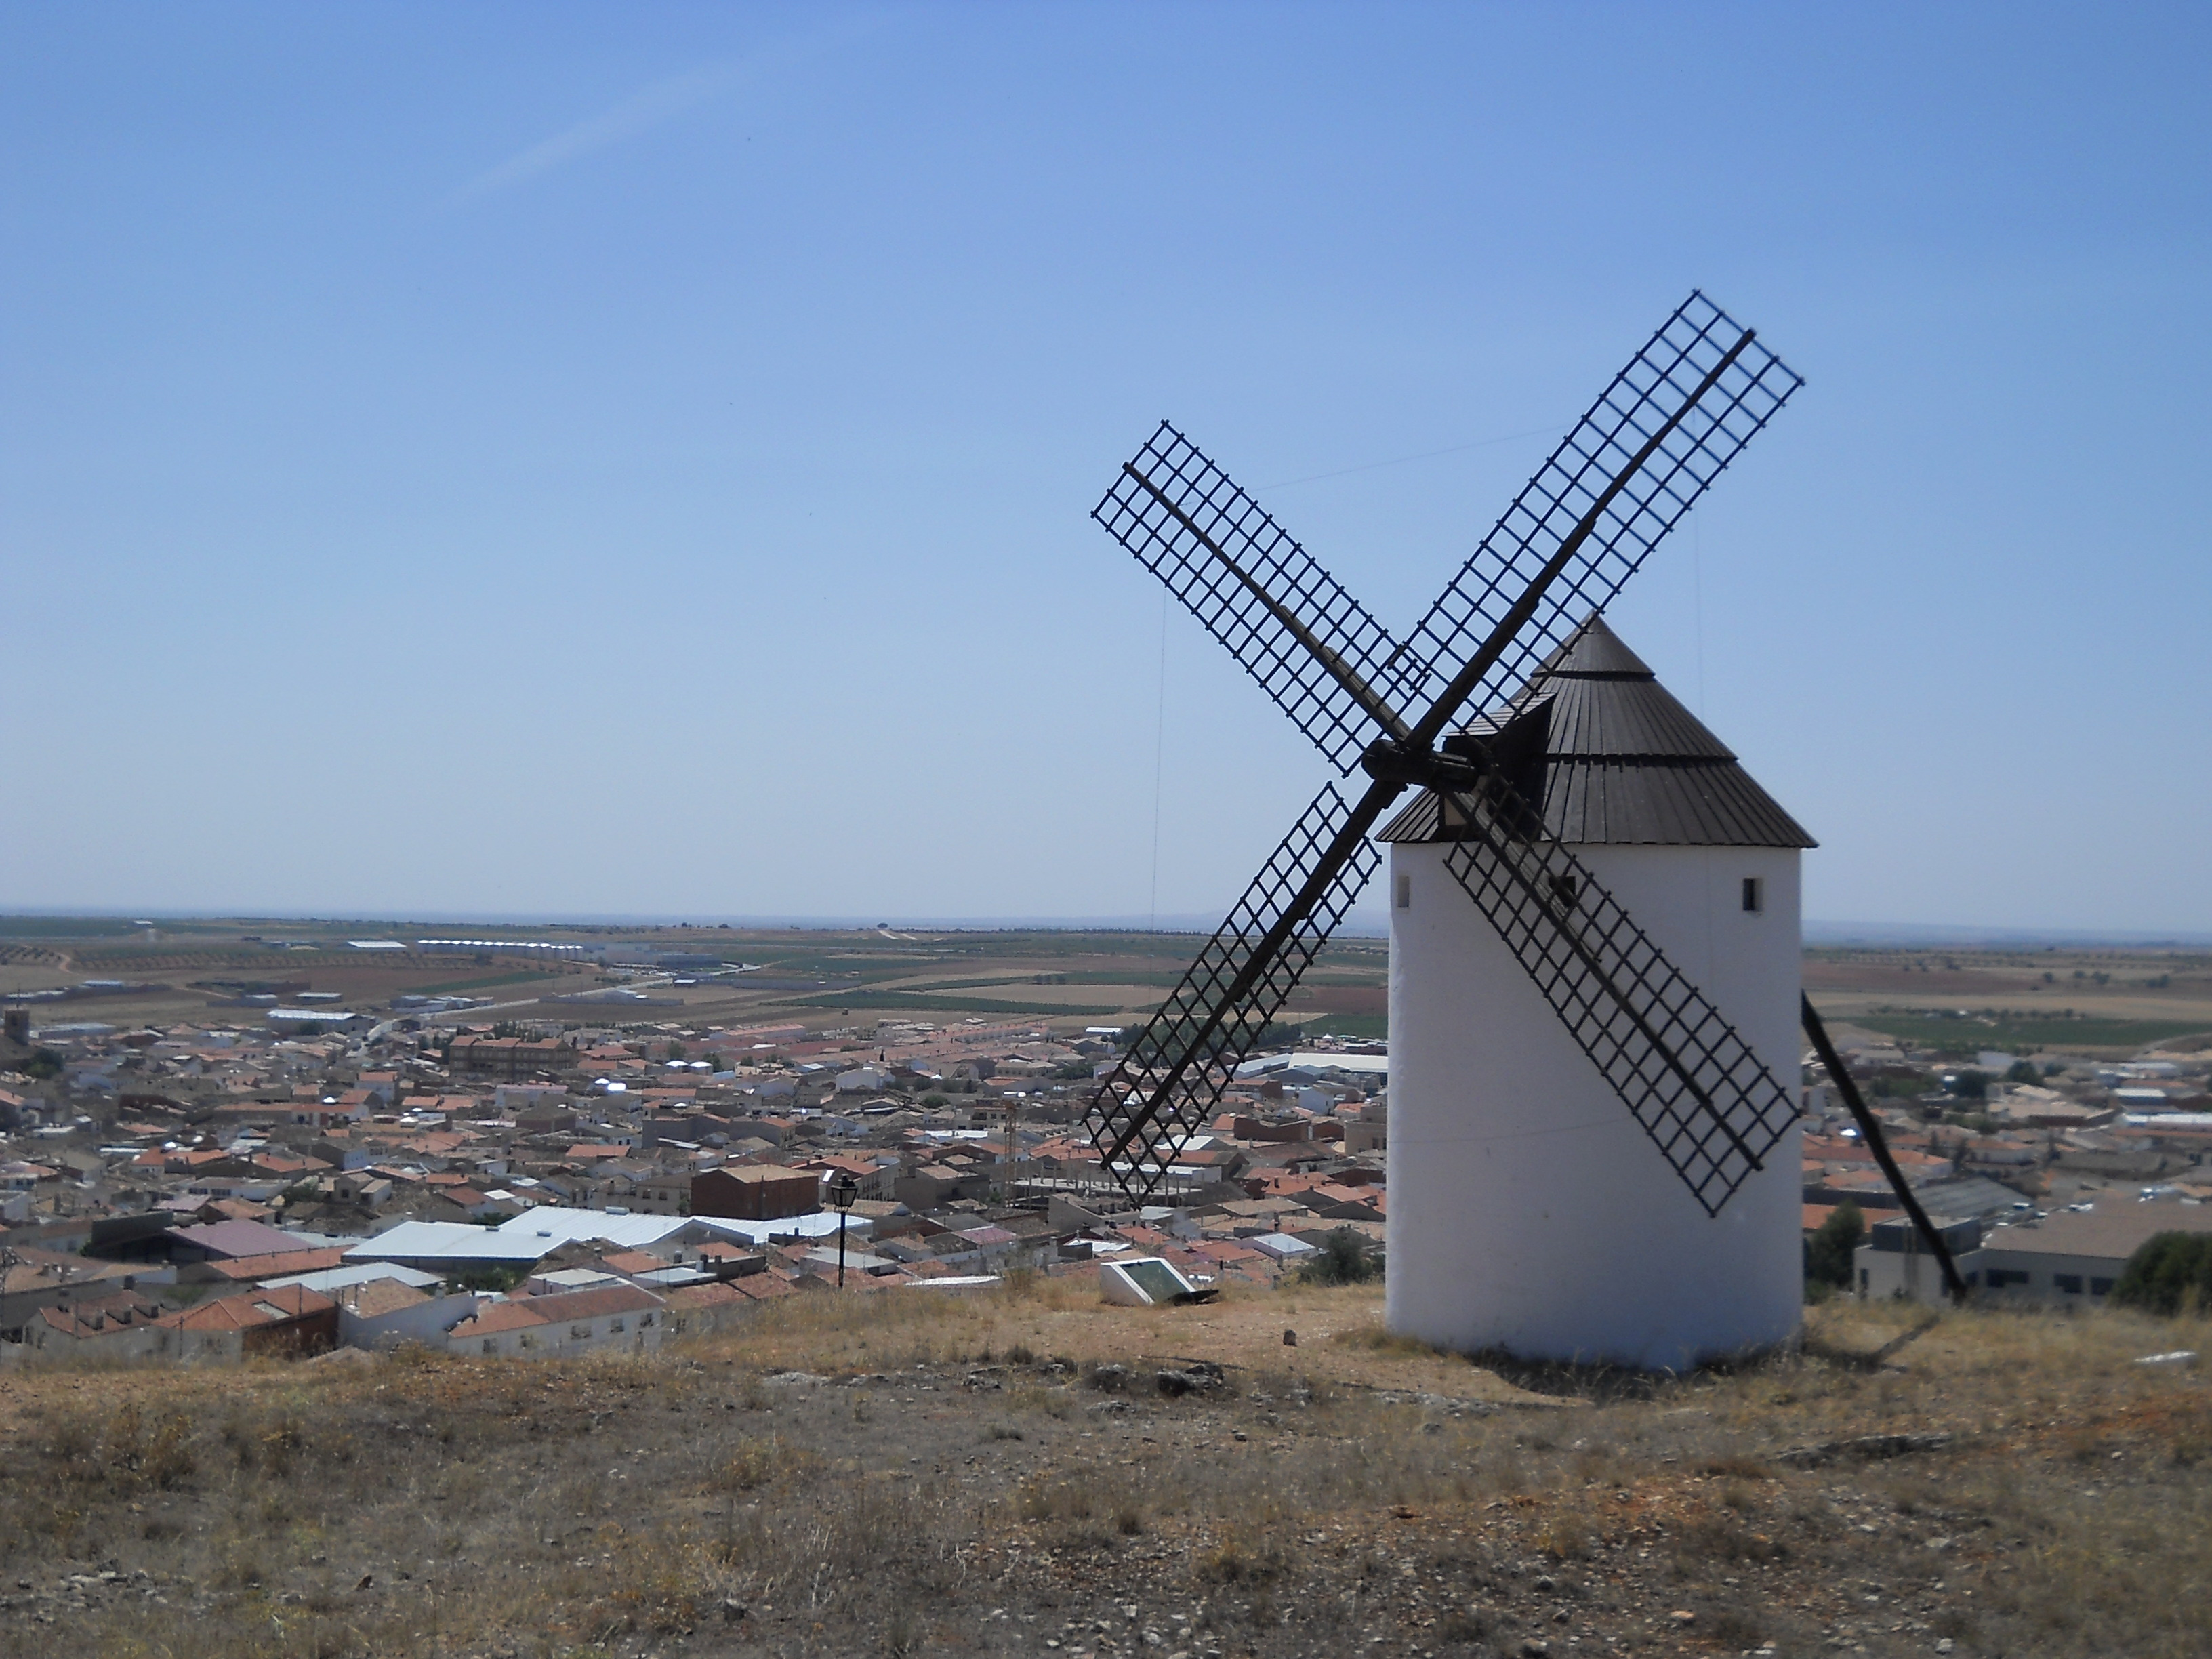
\includegraphics[width=0.45\textwidth]{img/molino.jpg}
	\caption{Distinguir el molino del pueblo del fondo no es difícil para un humano aunque sí para una máquina.}
	\label{img:ejemplomolino}
\end{figure}

\REV{pq es importante el problema de la segmentación} Autores como González y Woods en \cite{lib:gonzalez} enuncian el problema de ``segmentación de imágenes no triviales como una de las tareas más dificiles en el procesamiento de imágenes''. En este sentido, insisten en que ``la exactitud de la segmentación determina el éxito o error de los procesos de análisis computerizados''. Otros autores \cite{lib:sonka} hablan de la sementación como una ``técnica en al que se divide la imagen en partes que tienen una correlación con objetos o áreas del mundo real contenidas en la imagen''. Definido formalmente:

\begin{definition}\label{def:definicionproblema}
Dada una imagen $Q$ que se pude subdividir en $n$ regiones $R_{1}, \dots, R_{n}$, y sabemos que $P$ es una cierta propiedad booleana que cumplen todos los píxeles de la región $R_{i}, \forall  i=1,\dots ,n$, se deberá cumplir siempre que:
\begin{enumerate}
	\item $\bigcup_{i=1}^{n}R_{i}=Q$;
	\item En una región $R_{i}, \forall i=1,\dots ,n$ todos sus píxeles están conectados;
	\item $R_{i}\cap R_{j}=\emptyset, \forall i, j : i\neq j;$
	\item $P(R_{i}) = \text{ VERDADERO }, \forall  i=1,\dots ,n;$
	\item $P(R_{i}\cup R_{j}) = \text{ FALSO }, \forall  i=1,\dots ,n.$
\end{enumerate}
\end{definition}

En conclusión, en este proceso se lleva a cabo la división de la imagen en regiones donde cada una (desde 2 hasta $n$, este número dependerá del problema que estemos resolviendo) harán mención al fondo y a cada objeto. Además, todas las regiones serán independientes entre sí, esto es, un pixel pertenecerá solamente a la región $i$ cuando hablemos de segmentación completa. Centrando el problema únicamente en aquellas imágenes en escala de grises, nuestra pretensión será obtener aquellas regiones que contienen a un objeto centrándonos en sus tonalidades, esto es, por medio de técnicas de umbralización \REV{seguro?}.


% 1.3. SOLUCIÓN
\section{Solución propuesta}\label{sec:solucion}
\REV{Nosotros vamos a utilizar técnicas difusas, para empezar. ¿Por qué? (Incertidumebre en torno a los píxeles, péridda de información captación imágenes,...)}

Existen tres técnicas para poder llevar a cabo la segmentación de una imagen:
\REV{explicación y referencia}
\begin{enumerate}[label=\alph*)]
	\item Segmentación basada en umbralización.
	\item Técnicas basada en agrupamiento de píxeles en regiones.
	\item Técnicas basadas en la detección de bordes.
\end{enumerate}

En este trabajo se va a centrar la segmentación por medio de las técnicas de umbralización. Para ello lo que tendremos que hacer será calcular los umbrales que separen las regiones que se hayan encontrado, de forma que situaremos las regiones entre un umbral $t_{i}$ y uno $t_{i+1}$. Para ejemplificar esto, tomaremos la umbralización binaria en la cual se dispondrá de un único umbral $t$. De esta forma, todos los elementos de la imagen que se encuentren por encima del umbral pertenecerán a una región  y los que estén por debajo a la segunda. Esta técnica se basa únicamente en detectar los diferentes tonos de gris de la imagen, así que mirando el histograma de la imagen (fig. \ref{img:rice}, podríamos ver cómo existe una frontera entre la intensidad $t=71$ y el resto creando diferencias en los niveles de gris. \cite{art:refbarrenechea}

\begin{figure}
\centering
	\subfloat{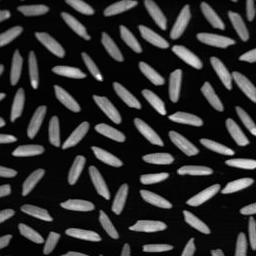
\includegraphics[width=0.3\textwidth]{img/rice}}
	\subfloat{
\includegraphics[width=0.3\textwidth]{img/umbra-rice}}\\
	\subfloat{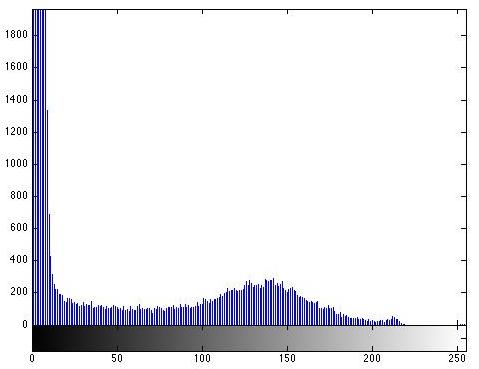
\includegraphics[width=0.4\textwidth]{img/hist-rice}}
	\caption{(a) Imagen original. (b) Imagen segmentada. (c) Histograma de la imagen original. Se puede ver que en t=71 se produce un mínimo con respecto a los otros niveles de gris y que por eso se escoge como umbral.}
	\label{img:rice}
\end{figure}


\REV{solución al pq...} Se debe tener en cuenta que la umbralización es un método rápido y de coste computacional bajo por lo que se puede realizar en tiempo real. Como sólo basa su algorítmica en el histograma de la imagen hace que sea una método sencillo e intuitivo aunque esto también hace que tenga problemas ante el ruido y objetos o fondos que no sean uniformes.

La solución que se presenta en este trabajor se haya por medio de lógica difusa. Se han utilizado funciones REF, de Dombi, de agregación y penalti. En el capítulo \ref{basicos} se hace mención a todos estos conceptos y se explican poníendose en práctica a partir del capítulo \ref{monoumbral}. En el capítulo \ref{cap:conclusiones} se presentan todas las conclusiones obtenidas así como las líneas de trabajo futuro.

%La umbralización es rápida, de coste computacional bajo y se puede realizar en tiempo real.
%Sencilla e intuitiva.
%Técnica útili si el fondo y los objetos son uniformes.
%Problemas: el ruido, niveles de gris similares entre obejto y fondo, solapamientos de objetos...
%La obtención de un umbral se basará en el histograma de la imagen. No se considera la información espacial.

% 1.4. REELEVANCIA
\section{Reelevancia}\label{sec:reelevancia}

En el campo de la medicina \cite{lib:suri} se ha experimentado una mejora sustancial en la efectividad de las pruebas médicas gracias a diferentes opciones como los rayos X, la tomografía computerizada, la resonancia magnética, la tomografía por emisión de positrones (PET), imágenes de ultrasonidos y otras. La revolución digital y el gran poder de procesamiento que disponen los ordenadores ha conseguido que los profesionales comprendan la compleja anatomía humana, aunque esto no ha sido suficiente ya que se ha visto necesario poder obtener los bordes, las superficies y la segmentación de los órganos. Estos órganos segmentados y sus bordes son clave para poder conseguir que un especialista médico pueda hacer una cirugía adecuada para muchas ramas de la medicina, debido a la importancia de tener datos en tiempo real. \REV{[Insertar figura que vaya con esto].}


Pruebas médicas
Localización de tumores y otras patologías
Medida de volúmenes de tejido
Cirugía guiada por ordenador
Diagnóstico
Planificación del tratamiento
Estudio de la estructura anatómica

Análisis automático de detección de errores.

Sensor de huella digital
Localización de objetos en imágenes de satélite (teledetección).
\REV{Alargar esto}


% 1.5. OBJETIVOS
\section{Propósito y objetivos}\label{sec:objetivos}

Este proyecto se centra en estudiar técnicas de segmentación para un único umbral y la generalización de estas en múltiples umbrales en imágenes en blanco y negro e intentar mejorar las técnicas de las que actualmente se disponen intentando generalizarlas de forma que los parámetros no dependan del problema. 

Además, para poder conseguir el propósito anterior se estipularon los siguiente objetivos:
\begin{itemize}
	\item Investigar y conocer técnicas actuales de segmentación de imagen de forma que estas sean el punto de partida.
	\item Analizar y evaluar las funciones que J. Dombi propone en \cite{art:dombi}. Comparar estas con las funciones REF y sustituirlas en la construcción de los conjuntos difusos para conocer sus efectos.
	\item Implementar diferentes algoritmos de segmentación con el conocimiento adquirido anteriormente evaluando su mejora y haciendo las correcciones necesarias con la intención de generalizar el método de forma máxima.
	\item Implementar diferentes algoritmos que incluyan la agregación de las diferentes funciones estudiadas para la segmentación en los puntos anteriores comprobando si esto mejora los resultados anteriores.
	\item Analizar todos los puntos anteriores a fin de concluir los resultados del trabajo así como dirimir si se ha podido conseguir cumplir el propósito inicial.
\end{itemize}

%1.6 ANÁLISIS BIBLIOGRÁFICO
\section{Análisis bibliográfico}
No tengo claro aun que poner aquí. Próximamente.

\chapter{Conceptos básicos}\label{preliminares}\label{basicos}

Este capítulo pretende ser una introducción a todos los conceptos teóricos necesarios para la correcta comprensión del trabajo que se detalla en esta memoria. 


\section{Procesamiento digital de imagen}\label{sec:procesamiento}
Un imagen $Q$ puede ser entendida como una función de dos variables, $q(x,y)$, donde $x$ e $y$ son las coordenadas en el plano de cada elemento (píxel) y la función da como resultado el nivel de gris o intensidad asociada a ese píxel. En concreto, cuando $x$ e $y$ así como la intensidad $q(x,y)$ son finitas y discretas hablaremos de que tenemos una imagen digital. Por eso mismo, el procesamiento digital de imagen se puede definir como aquel que se hace con imágenes digitales a través de un ordenador. Tiene su origen con la introducción de las primeras imágenes digitales a principios de 1920, donde se enviaban imágenes entre Londres y Nueva York por medio de un cable submarino.

Es claro que los seres humanos disponemos del sentido de la vista como el sentido más desarrollado para interacturar con el medio, pero esta está limitada a la banda visible dentro del espectro electromagnético. En cambio, el procesamiento digital de imagen puede cubrir el análisis de todo el espectro electromagnético, lo que incluye los ultrasonidos, el infrarrojos, rayos X, etc. Esta es la principal razón por la que el procesamiento digital de imagen puede incluirse en una gran cantidad de campos.\REV{quitar ultima frase?}

Dentro del procesamiento de imagenes digitales se encuentra la visión artificial. Esta es una subcampo de la inteligencia artificial (IA) y pretende emular la visión humana, incluyendo la capacidad de aprender así como el manejo directo de imágenes como datos de entrada a un problema dado. Actualmente, este campo está poco desarrollado \cite{lib:gonzalez} ya que el avance está siendo mucho más lento de lo que se esperaba en un primer momento. El análisis de imagen, que pretende entender cómo está formada la imagen, está situada a caballo entre la visión artificial y el procesamiento de imágen, y será lo que utilizaremos en este trabajo.

No hay una clara frontera entre el procesamiento de imagen y la visión artificial, esto hace que se hable de un paradigma que incluye 3 tipos de procesos; de bajo nivel, medio nivel y alto nivel. Dentro del nivel bajo se pueden incluir todos los procesos primitivos que tienen como objetivo reducir el ruido, realzar el contraste o ajustar la nitidez, por ejemplo. En un segundo nivel, más avanzado, se encuentran todos los procesos que tienen como entrada una imagen y obtienen atributos de esta. Pueden ser procesos como la segmentación (que se tratará aquí), descripción de objetos de la imagen o recocimiento de los mismos. En el último nivel se encuentran todas aquellas técnicas que hacen que todo ``tenga sentido'' ya que hacen que el análisis imite a la forma cognitiva de la mente humana.


\subsection{Imágenes digitales}\label{sec:imagenesdigitales}
Como ya se ha explicado en el apartado anterior, se habla de imagen digital cuando se puede ser capaz de determinar todos sus elementos (píxeles), es decir, estos son de forma finita y discreta. A partir de esta idea, se dispone de dos formas de representación para las imágenes en niveles de gris, en los rangos $[0,1]\in\RR$ y $[0,255]\in\NN$. En el primer caso diremos que la imagen está normalizada. Además, las imágenes digitales serán representadas por una matriz que contendrá cada uno de sus píxeles de manera ordenada.


\begin{figure}
\centering
    \subfigure[Niveles de gris]
    {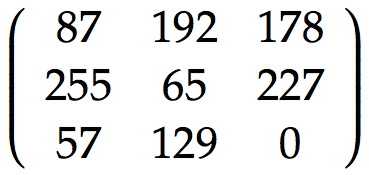
\includegraphics[height=0.1\textwidth]{img/matriznivelesgris.jpg}}\quad
    \subfigure[Normalizada]
    {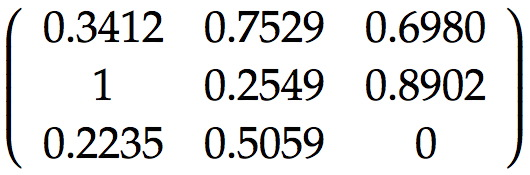
\includegraphics[height=0.1\textwidth]{img/matriznormalizada.jpg}}\quad\ 
    \subfigure[Gráfica]
    {
\includegraphics[width=0.1\textwidth]{img/imagendigital.jpg}}
    \caption{Imagen digital en diferentes representaciones.}
    \label{fig:defimagen}
\end{figure}

Como se puede apreciar en la figura \ref{fig:defimagen} cuanto más cercano a 0 sea el número, más negro será el nivel de gris, y cuanto más cercano a 1 ó 255, más blanco. En el caso de imágenes en color, se utiliza el formato RGB ({\em Red}, {\em Green} y {\em Blue}) donde existe una matriz como las anteriores por cada uno de los colores y al superponerlas se obtiene la imagen que vemos habitualmente.

\begin{definition}\label{def:histograma}
Se define el histograma de una imagen $Q$ con niveles de gris en el intervalo [0, 255] como la función $h(q) = n_q$ donde $n_q$ es el número de píxeles en la imagen con la intensidad $q$.
\end{definition}

Un ejemplo gráfico de la función de histograma para una imagen puede encontrarse en la figura \ref{img:rice}.


\subsection{Herramienta para el procesamiento digital: \MATLAB}\label{sec:matlab}
\MATLAB\ (abreviatura de {\em Matrix Laboratory}) es una herramienta de software matemático que ofrece un lenguaje de programación (lenguaje M) y un entorno de desarrollo integrado. Fue creado en 1984 por el informático y matemático Cleve Moler el cual buscaba una forma alternativa de ejecutar programas de álgebra en {\em Fortran}.

Entre sus prestaciones básicas están la manipulación de matrices, la representación de datos y funciones o la implementación de algoritmos así como la creación de interfaces de usuario (GUI). Además, el paquete básico de \MATLAB\ puede ser expandido por medio de {\em toolboxes}, como es el caso de este trabajo, donde se utilizará la relativa  a procesamiento de imagen. Se puede disponer también del software {\em Simulink} para trabajar conjuntamente a \MATLAB.

\subsection{Contraste}
Como en el trabajo se hace uso de imágenes con alto y bajo contraste, disponer una pequeña explicación. Pillar de los libros del laboratorio. \REV{Revisar}.

\subsection{Ruido en las imagenes}\label{sec:ruido}
Se condidera que una imagen está degradada cuando tiene ruido, esto es, cuando tiene defectos con respecto a la imagen original (fig. \ref{fig:defruido}). La principal fuente de ruido en images digitales se da en la adquisición o transmisión de las imagenes. Esto se puede deber a las condiciones ambientales o a la calidad de los sensores durante la toma de la imagen. Por ejemplo, la luminosidad, el polvo en el ambiente, etc. pueden ser determinantes. Por otra parte, en el caso de la transmisión, las imágenes pueden ser corrompidas por interferencias en el medio de transmisión, principalmente. Esto es claro cuando se transmite una imagen de un satélite, ya que la atmósfera interferir y provocar que la imagen recibida en la base terráquea no sea exactamente igual.
\begin{figure}
\centering
    \subfigure[Imagen original]
    {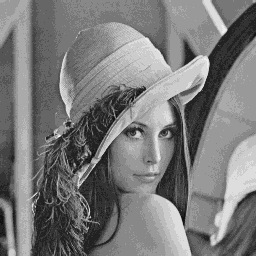
\includegraphics[width=0.3\textwidth]{img/lena}}\quad
    \subfigure[Imagen con ruido `sal y \mbox{pimienta}']
    {
\includegraphics[width=0.3\textwidth]{img/lenas&p}}\quad
    \subfigure[Imagen con ruido gausiano]
    {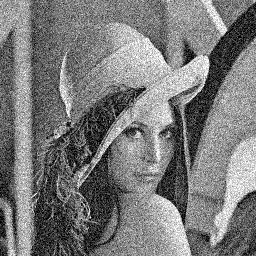
\includegraphics[width=0.3\textwidth]{img/lenaga}}
    \caption{Imagen de Lena con diferentes tipo de ruido}
    \label{fig:defruido}
\end{figure}

Las imágenes con ruido también se pueden crear artificialmente. Para ello utilizamos una cierta función $H$ de degradación, a la que añadimos un ruido al que llamaremos $\eta$ de forma que obtendremos una nueva imagen $g(x,y)$ que tendrá una serie de imperfecciones. Todo el ruido creado de esta forma se aplicará directamente sobre los píxeles de la imagen lo que provocará cambios en su histograma en una forma u otra. Aun así, debemos tener en cuenta que no hay relación directa entre la intensidad nueva que tienen los píxeles y la anterior. 

Existen muchos tipos de ruido como el exponencial, el gamma, el uniforme, etc. pero en esta memoria se han utilizado, el gausiano y el de tipo impulsivo o de `sal y pimienta'.

\subsubsection{Ruido gausiano}
Este puede ser uno de los modelos de ruido más utilizado en la práctica debido a que tiene una gran maleabilidad matemática. Basa su forma de actuar sobre la imagen en la función gausiana de probabilidad:
$$p(z) = \frac{1}{\sqrt{1}{2\pi\sigma}} e^\frac{-(z-\mu)^2}{2\sigma^2}$$
donde $z$ representa la intensidad, $\mu$ la media de $z$ y $\sigma$ la desviación estándar. Este tipo de ruido puede crearse en \MATLAB\ a través de la función \mintinline{matlab}{imnoise(img_var, 'gaussian')} sabiendo que \mintinline{matlab}{img_var} es la variable donde está almacenada la imagen en tipo \mintinline{matlab}{uint8}.

\subsubsection{Ruido de tipo `sal y pimienta'}
Este tipo de ruido, formalmente llamado impulsivo, hace que se conviertan píxeles de forma aleatoria en píxeles con intensidad 0 y 255. Esta es la razón de su particular nombre. De nuevo, fijándonos en \MATLAB, podremos crear imágenes con este tipo de ruido por medio del comando \mintinline{matlab}{imnoise(img_var, 'salt & pepper', prob_val)}, de nuevo \mintinline{matlab}{img_var} es la variable donde se almacena la imagen y \mintinline{matlab}{prob_val} es un valor entre 0 y 1 que hace las veces de probabilidad de la aparición del ruido. 

En este trabajo, se han utilizado imágenes con ruido para comprobar la adecuación o no de los algoritmos de segmentación al ruido. Ejemplos de ambos tipos de ruido se han presentado en la figura \ref{fig:defruido}.


% LOGICA DIFUSA
\section{Lógica difusa}\label{sec:logicadifusa}
La lógica difusa fue introducida por el matemático L. A. Zadeh \cite{art:zadeh} en 1965 con la intención de poder extender la lógica clásica o {\em crips} de forma que permitiera manejar y procesar la información que se compone de términos inexactos, imprecisos o subjetivos. Es, al fin y al cabo, un intento de imitar la forma de deducción del cerebro humano para trasladarlo a las máquinas. Se comenzará recordando la lógica clásica para después extender los conceptos a la difusa.

En primer lugar, definiremos el universo finito, $U$,  con el que se  trabajará, de forma que contenga todos aquellos elementos con los que se desee trabajar, esto es, $U = \{u_{1}, u_{2}, \dots, u_{n}\}$. En la lógica clásica simplemente asignamos verdadero o falso a cada uno de los elementos del conjunto que se estudia. Por esta razón, al definir un conjunto $A$ podremos decir que este contiene o no a los elementos del universo $U$ con una certeza absoluta. De esta manera, daremos un valor de 1 cuando $u_{i}$ esté incluido en $A$ (verdadero) y un valor de 0 cuando no lo esté (falso). En esta última idea se refleja por medio de la función de pertenencia al conjunto  $A$, $\mu_{A}$ (ecuación \ref{eq:logicaclasica}).
\begin{equation}\label{eq:logicaclasica}
\begin{aligned} 
	A = \{(u_{i}, \mu_{A}(u_{i})) | u_{i}\in U\}\\
	\mu_{A}:U\rightarrow \{0,1\} \text{ tal que}\\
	\mu_{A}(u) = \left\{ \begin{aligned}
		1 \quad\text{si}\quad u\in A\\
		0 \quad\text{si}\quad u\notin A
 	\end{aligned}\right.
\end{aligned}
\end{equation}
%\REV{revisar ecuación con respecto al ejemplo} Se da más adelante la concreta.

 Podemos considerar el problema de determinar si una persona es alta o no. Para la lógica clásica, este razonamiento se simplificará en buscar un valor a partir del cual podamos definir que cierta persona es alta. Para el siguiente ejemplo, tomaremos 1,75 metros como referencia, donde $A$ es el conjunto de las personas altas. De este modo, $\mu_{A}=1 \text{ si } u>1,75$ y en otro caso $\mu_{A}=0$. En la figura \ref{fig:altoclasica} se puede ver la representación del concepto `alto' para las posibles alturas que se pueden presentar.

\subfile{graficos/logicaclasicagraf}

Por otra parte, la lógica difusa dispone de la función de pertenencia más compleja, lo que nos hace poder decir que alguien es `poco alto' o `bastante alto' ya que no daremos un par de valores ($\{0,1\}$) sino cualquiera de los contenidos en el intervalo que definen. Así $\mu_{A}$ será una función que asigna un valor entre 0 y 1 a cada elemento de $A$.\begin{equation}\label{eq:logicadifusa}
\begin{aligned} 
	A = \{(u_{i}, \mu_{A}(u_{i})) | u_{i}\in U\}\\
	\mu_{A}:U\rightarrow [0,1]
\end{aligned}
\end{equation}                
Si continuamos con el ejemplo se verá que el conjunto alto ($A$) esta vez se define como explica la ecuación \ref{eq:ejemplodifusa}. 

\begin{equation}\label{eq:ejemplodifusa}                
	\mu_{A}(u) = \left\{ \begin{aligned}
		1 \quad&\text{si}\quad u\geq 2\\
		2u - 3 \quad&\text{si}\quad 1.5>u>2\\
		0 \quad&\text{si}\quad u\leq 1.5
 	\end{aligned}\right.
 \end{equation}           
Esta nueva función de pertenencia hace que podamos distinguir 3 zonas dentro de su representación (figura \ref{fig:altodifusa}). Se tendrá de nuevo la etiqueta `alto' y `no alto' que hacen que su pertenencia sea certera. Se dispondrá, también, una parte de la pertenencia a la que llamaremos `difuso' donde el conjunto no afirma ser ni `alto' ni `no alto' sino que está en una situación intermedia. En este caso se habla de que el elemento $a_{i}$ que se encuentra ahí pertenece a $A$ con grado $\mu_{A}(a_{i})$.
                
\subfile{graficos/logicadifusagraf}

Más formalmente, denotaremos al conjunto que incluye a todos los conjuntos difusos como $\FF(u)$ a todos aquellos que se encuentran definidos sobre un referencial finito ($|U| = n$) por lo que $U$ no será un conjunto vacío.
 


% FUNCIONES REF
\section{Funciones de equivalencia restringida (REF)}\label{sec:ref}
El concepto de función de equivalencia restringida (REF por sus siglas en inglés) surge del concepto de equivalencia y el de similitud \cite{art:refbarrenechea}. Este concepto es muy utilizado para la comparación de imágenes y su intención es dar una medida de cómo de iguales o similares son dos elementos $x$ e $y$. Para poder definir el concepto de REF, necesitamos varios previamente. 

\begin{definition}\label{def:negacionestricta}
Una negación estricta es aquella función $c : [0, 1] \rightarrow [0, 1]$ que cumple que $c(0)=1$ y $c(1)=0$ y es estrictamente decreciente y continua. Además, si $c$ es involutiva se considera que se habla de una negación fuerte.
\end{definition}

\begin{definition}\label{def:automorfismo}
Llamaremos automorfismo ($\varphi$) a todas aquellas funciones del intervalo unidad tal que $\varphi : [0, 1] \rightarrow [0, 1]$ sean continuas y estrictamente crecientes propiciando que $\varphi(0)=0$ y $\varphi(1)=1$.
\end{definition}

En 1979, E. Trillas \cite{art:thtrillas} enunció el siguiente teorema. 
\begin{theorem}[Teorema de Trillas]\label{th:trillas}
Una función $c : [0, 1] \rightarrow [0, 1]$ es una negación fuerte si, y sólo si, existe un automorfismo del intervalo unidad tal que $c(x)=\varphi^{-1}(1-\varphi(x))$.
\end{theorem}

\begin{definition}\label{def:ref}
Una función $REF  : [0, 1] \rightarrow [0, 1]$ es llamada de equivalencia restringida cuando cumple que:
	\begin{enumerate}
	\item $REF(x, y) = REF(y, x), \forall x, y \in [0, 1];$
	\item $REF(x, y) = 1$, si y sólo si, $x=y$;
	\item $REF(x, y) = 0$, si y sólo si, $x=1$ e $y=0$ ó si $x=0$ e $y=1$;
	\item $REF(x, y) = REF(c(x), c(y)),  \forall x, y \in [0, 1]$, siendo $c$ una negación fuerte.
	\item $\forall x, y, z \in [0, 1]$, si $x\leq y\leq z$, entonces $REF(x, y)\geq REF(x, z)$ y  $REF(y, z)\leq REF(x, z)$
	\end{enumerate}
\end{definition}

\begin{proposition}\label{prop:contruccionref}
Sean dos automorfismos $\varphi_{1}$ y $\varphi_{2}$, se llamará función $REF$ a la construcción que cumpla que: 
$$REF(x,y) = \varphi_1^{-1}(1-|\varphi_2(x)-\varphi_2(y)|) \quad\text{con}\quad c(x) = \varphi_2^{-1}(1-\varphi_2(x)).$$ 
Además, si tenemos una $REF$ y un automorfismo en $\unitinterval$, la aplicación de estos ($F=\varphi \circ REF$) es otra $REF$.
\end{proposition}

\begin{theorem}\label{th:ref}
Una función continua $REF:\unitinterval^2 \rightarrow\unitinterval$ que cumpla que $REF(1,x)=x, \xinunitinterval$, es una función $REF$ asociada con la función $I:\unitinterval^2\rightarrow\unitinterval$ con $I$ continua y asociativa si y sólo si existe un automorfismo $\varphi$ en $\unitinterval$ tal que:
$$REF(x,y)=\varphi^{-1}(1-\abs{(\varphi(x)-\varphi(y))})\quad\text{ y }\quad c(x)=\varphi^{-1}(1-\varphi(x))$$
\end{theorem}

%\REV{Teorema que hace que estos automorfismos puedan ser 1 solo?} No lo pongo pq no lo utilizo.


% FUNCIONES DE AGREGACIÓN
\section{Funciones de agregación}\label{sec:agregacion}
%\REV{funciones de agregación vs operadores de agregación ¿Qué es más correco para nombrarlos?} -> Funciones de agregación.
Las funciones de agregación tienen como propósito reducir las dimensiones de la información a partir de la combinación de los datos de entrada obteniendo una salida que los represente \cite{art:montero, art:calvoagregacion}. Su aplicación se extiende en muchos casos prácticos y teóricos como la lógica multievaluada, control difuso, la toma de decisión, etc \cite{art:paternain}.  Se definirá una función de agregación como sigue:

\begin{definition}\label{def:agregacion}
Se dice que $M : \unitinterval^n \rightarrow \unitinterval$ es una función de agregación de dimensión $n$ siempre que satisfaga:
	\begin{enumerate}
	\item $M(x_1, \dots, x_n) = 0$ si y sólo si $x_1=\dots=x_n=0$;
	\item $M(x_1, \dots, x_n) = 1$ si y sólo si $x_1=\dots=x_n=1$;
	\item $M$ es una función estrictamente creciente.
	\end{enumerate}
\end{definition}
\begin{definition}
Una función de agregación $M$ será llamada media si
$$ \min(x_{1}, \dots, x_{n})  \leq M(x_{1}, \dots, x_{n}) \leq \max(x_{1}, \dots, x_{n}).$$
\end{definition}

En este proyecto se utilizarán mayoritariamente las funciones de agregación idempotentes, esto es, que cumplen que $M(x,\dots ,x)=x, \forall x$. En particular, una función de agregación idempotente es una media. Entre las funciones que utilizaremos encontramos la media aritmética, el mínimo, el máximo o la media geométrica. Además, se definen a continuación otras que no son de uso tan común.
% OWA
\subsection{Funciones OWA}
En esta sección se introduce el concepto de las funciones de media ponderada ordenada (OWA, {\em  ordered weighted averaging}) \cite{art:yagerowa, art:paternain, art:bustinceowa}. Se basan en la idea de generar una media, ordenando primero los elementos a agregar, para luego darles mayor relevancia a una parte de ellos. Este tipo de función generaliza la media aritmética, siendo esta el OWA en el que todos los elementos del vector de pesos son iguales.

\begin{definition}\label{def:owa}
Una  función $F:\unitinterval^n\rightarrow\unitinterval$ será una función OWA de dimensión $n$ si existe un vector $w=(w_{1},w_{2},\dots,w_{n})\in \unitinterval^{n}$ tal que $\sum_{i}w_{i}=1$ de forma que
$$F(x_{1},\dots,x_{n})=\sum^{n}_{j=1}w_{j}x_{\sigma(j)}$$
donde $x_{\sigma(j)}$ es el $j$-ésimo mayor elemento del vector $(x_{1},\dots,x_{n})$.
\end{definition}

Por tanto para poder obtener un resultado adecuado, deberá utilizarse un vector de pesos $w$ que se adecúe a las necesidades del problema. En este trabajo se emplea la versión `al menos la mitad' %\REV{nombre}. Solucionado.
 que tiene como vector de pesos aquel que se obtiene con la ecuación \ref{eq:pesosowamayoria}. Esto generará una agregación donde destaquen todos aquellos elementos que se encuentren por detras de la mediana.
% a $w=(w_{1}\dots w_{i}, w_{i+1}\dots w_{n})$ sabiendo que $\abs{1, \dots, i}=\abs{i+1,\dots,n}$ de forma que $w_{j}=\frac{1}{2n}$ si $1\leq j\leq i$ y $w_{j}=0$ en el resto de los casos.\REV{buscar la versión buena, esto es sólo para los cardinales pares}.\REV{volver a redactar. Incluir construcción.}

\begin{equation}\label{eq:pesosowamayoria}
	 w_i = Q\left(\frac{i}{t+1}\right) - Q\left(\frac{i+1}{t+1}\right), \forall i\in \{1, \dots, n\}, \text{   sabiendo que}
\end{equation}
	 $$Q(r) = \left\{\begin{aligned}
	 	0 					&\quad \text{si}\quad r<0,5\\
	 	\frac{r-0,5}{0,5}	&\quad \text{si}\quad 0,5\leq r\leq 1\\
	 	1 					&\quad \text{si}\quad r>1\\
	\end{aligned}\right.$$
\REV{forma ecuación}

%\REV{reescrito}
Además, en la segunda parte del estudio, se emplea el OWA `la mayoría de'. Este OWA pretende destacar aquellos elementos que son mayores en el vector $x$. Esto se hace realidad por medio de un vector de pesos donde son nulos los pesos relativos a aquellas $x_i$ más pequeñas. Para la construcción del vector de pesos, se utilizará, también, la ecuación \ref{eq:pesosowamayoria}



% CHOQUET
\subsection{Integral Choquet}
Para este otro tipo de función \cite{art:choquet, art:sugenochoquet} de agregación se pretende dar una nueva de forma de representar un conjunto de datos en una única salida. De esta forma, se define primeramente una medida a través de la cual se calculará la forma en la que cada elemento del conjunto de datos tendrá reelevancia en la agregación final. Para ello definimos el concepto de medida difusa.
\begin{definition}\label{def:medidadifusa}
Dado $U$ un universo finito; $\mathcal{P}(U)$ el conjunto de todos los subcojuntos de $U$. Una medida difusa es una función $\mu:\mathcal{P}(U)\rightarrow\unitinterval$ que satisface que:
\begin{enumerate}
	\item $\mu(\emptyset)=0$ y $\mu(U)=1$.
	\item $A\subseteq B \Rightarrow \mu(A)\leq\mu (B), \forall A, B \subseteq U$.
\end{enumerate}
\end{definition}

A continuación definimos la función integral Choquet conociendo que tomaremos su versión discreta por el contexto en el que se está trabajando.

\begin{definition}\label{def:choquet}
Dado un vector $(x_1,\dots,x_n)$, sea $\sigma$ una permutación de $\{1,...,n\}$ tal que $x_{\sigma(j)}$ es el $j$-ésimo mayor elemento del vector $(x_{1},\dots,x_{n})$. La integral discreta de Choquet con respecto a la medida difusa $\mu$ es 
$$Ch_{\mu}(x)=\sum_{i=1}^{n}x_{\sigma(i)}(\mu(\{\sigma(i),\dots,\sigma(n)\})-\mu(\{\sigma(i+1),\dots,\sigma(n)\}))$$
tomando la convención de que $\{\sigma(n+1),\sigma(n)\}=\emptyset$.
\end{definition}

\begin{proposition}\label{prop:choque2owa}
Si denotamos a $w_{\sigma, i}^{\mu} = \mu(\{\sigma(i),\dots,\sigma(n)\})-\mu(\{\sigma(i+1),\dots,\sigma(n)\})$ se obtiene la siguiente definición de la integral Choquet en función de los operadores OWA definidos en \ref{def:owa}:
$$\sum_{i=1}^{n} w_{\sigma, i}^{\mu} \cdot x_{\sigma(i)}.$$
\end{proposition}


% FUNCIONES DE SIMILITUD
\section{Funciones de similitud}\label{sec:similitud}
El concepto de similitud \cite{art:fan1, art:fan2} surge cuando queremos medir cómo de parecidos son dos conjuntos difusos. Este concepto es muy parecido al de REF, pero en este caso se consideran conjuntos y no elementos. Por esta razón, utilizamos las REF como base para definir las funciones de similitud.
\begin{definition}\label{def:similitud}
Dada una función $M$ de agregación (definición \ref{def:agregacion}) y una función $REF$ (definión \ref{def:ref}) llamaremos a $SM$ función de similitud si $SM : \FF(X) \times \FF(X) \rightarrow [0,1]$ está definida tal que 
$$SM(A,B)=M^n_{i=1}REF(\mu_A(x_i), \mu_B(x_i))$$
y satisface las siguientes condiciones:
	\begin{enumerate}
	\item $SM(A, B) = SM(B, A), \forall A, B \in \FF(X)$;
	\item $SM(A, A_c) = 0$, si y sólo si A no es difuso;
	\item $SM(A, B) = 1$ si y sólo si A = B;
	\item Si $A\leq B\leq C$, entonces $SM(A, B)\geq SM(A,C)$ y $SM(C, B)\geq SM(C,A)$;
	\item $SM(A_c, B_c) = SM(A,B)$
	\end{enumerate}	
\end{definition}

\begin{remark}\label{obs:funcionesref}
Durante el desarrollo de este trabajo se buscará la similitud entre conjuntos difusos y el conjunto $\tilda1$. Se define el conjunto $\tilda1 =\{(u_{i}, \mu_{\tilda1}(x)=1)|u_{i}\in U \}$, esto es, aquel en el que todos sus elementos tienen pertenencia absoluta.
\end{remark}


% FUNCIONES PENALTI
\section{Funciones penalti}\label{sec:penalti}
Una función penalti  \cite{art:calvo} es una función de agregación, por lo que dispone de un vector de entradas del que devuelve un único resultado. Si todos los elementos del vector son iguales, entonces, claramente, la salida será eso mismo. Ahora bien, el problema surge cuando hay algún elemento diferente ya que en ese momento la idea será buscar una salida todo lo parecida posible a la entrada. En este sentido, es elemento o elementos diferentes tendrán una cierta discrepancia con los demás y justamente esto es lo que se pretende minimizar, la discrepancia, para dar una salida adecuada. 

\begin{definition}\label{def:penalti}
La función $P:[a,b]^{n+1}\rightarrow \RR^{+} = [0, \infty]$ es una función penalti si y sólo si satiface que:
\begin{enumerate}
	\item $P(x, y) \geq 0, \forall x, y$
	\item $P(x, y) = 0$ si $x_{i}=y \forall i=1,\dots ,n$
	\item $P(x,y)$ es cuasiconvexa en $y$ para cualquier $x$, esto es, $P(x, \lambda\cdot y_{1} +(1-\lambda)\cdot y_{2})\leq \max(P(x, y_{1}), P(x, y_{2}))$.
\end{enumerate}
\end{definition}
La función en la que se basan las penalti es $$f(x)=\arg\min_{y} P(x,y)$$ si $y$ es el único mínimo e $y=\frac{a+b}{2}$ si el conjunto de minimizadores es el intervalo $(a, b)$.

\begin{theorem}
Todas las funciones de agregación llamadas medias pueden ser escritas como una función basada en una función penalti expresada en la definición \ref{def:penalti}.
\end{theorem}


% FUNCIONES DE DOMBI
\section{Funciones de Dombi}\label{sec:dombi}
Las funciones de Dombi \cite{art:dombi} son operadores de equivalencia con una definición diferente a las REF presentadas en la sección \ref{sec:ref}. Con esta relación lo que se pretende conocer es como de iguales son dos elementos de un conjunto difuso dado, pero aplicando nuevas ideas para la construcción del resultado. 
%\REV{Definición completa?} Pues así se va a quedar.
\begin{definition}\label{def:dombi}
Dados $x=(x_1, x_2, \dots,x_n)$ y $w=(w_1,w_2,\dots,w_n)$, denotaremos $D$ como una función de equivalencia de Dombi cuando tengamos que 
$$D(w,x)=\frac{1}{2}\left(1+\prod(1-2x_{i})^{w_{i}}\right)$$
\end{definition}
\begin{lemma}\label{def:propiedadesdombi}
La función de equivalencia de Dombi, $D$, cumple las siguientes propiedades:
\begin{enumerate}
	\item $D:\unitinterval\times\unitspace \text{ es continua}$;
	\item $D((w_1,w_2),(0,0)) = 1$;\quad$D((w_1,w_2),(1,1)) = 1$;
	\item $D((w_1,w_2),(0,1)) = 0$;\quad$D((w_1,w_2),(1,0)) = 0$;
	\item $D((w_1,w_2),(x,c(x))) = 0$.
\end{enumerate}
\end{lemma}
%\REV{propiedades}



%NOTACIÓN
\section{Notación}\label{sec:notacion}

A lo largo del trabajo se asumirá la notación que sigue para estos conceptos.

\begin{description}
    \item[Imagen]: la denotaremos con $Q$.
    \item[Coordenadas de un pixel]: $(x,y)$.
    \item[Máximo nivel de gris]: $L$.
    \item[Número de filas de $Q$]: $N$.
    \item[Número de columnas de $Q$]: $M$.
    \item[Intensidad de un pixel]: $q(x,y)$ de forma que $0\leq q(x,y)\leq L-1, \forall (x,y)\in Q$.  
    \item[Histograma]: $h(q)$. Función para conocer el número de pixeles con la intensidad $q$. 
    \item[Media de una imagen]:$$m_Q=\frac{\sum_{q=0}^{L-1}qh(q)}{\sum_{q=0}^{L-1}h(q)}$$
    \item[Área de una imagen]: $$A(Q) = \sum_{q=0}^{L-1} q h(q)$$
\end{description}


\chapter{Segmentación de imágenes con un solo umbral}\label{monoumbral}
a
\chapter{Segmentación de imágenes con agregando con funciones OWA}

En este capítulo se llevarán a cabo otro tipo de pruebas sobre los algoritmos presentados. Para ello, en primer lugar, se explicará el modo en el que se modificarán los algoritmos presentados en la sección \ref{sec:algoritmosmono}. Después se presentarán los resultados obtenidos con estas fórmulas, haciendo hincapié en los más interesantes.

%\section{Métodos algorítmicos de segmentación de un único umbral}
%\REV{Añadir todos aquellos detalles teóricos necesarios a tener en cuenta para continuar con los experimentos.}
%\input{contenidos/4-1-algoritmos}

\section{Experimentos y resultados con funciones de agregación OWA}

% EXPERIMENTO 4
\subsection{Experimento 4: sustitución de la media aritmética por funciones OWA en la construcción de los conjuntos difusos}
Para todos los experimentos que se disponen en este capítulo, tomaremos la determinación de sustituir la media aritmética que se utiliza en la construcción de los conjuntos difusos (def. \ref{def:mediasmonoumbral} y \ref{def:conjuntodifusomonoumbral}) por una función OWA de tipo `la mayoría de' (def. \ref{def:owa}). Para ello es importante destacar el hecho de que habrá que introducir todos los datos en forma normalizada (con valores en $[0,1]$).

En concreto, se utilizarán dos posibilidades de funciones OWA. La primera de ellas, OWA (1), crea los pesos según la ecuación \ref{eq:pesosowamayoria} habiendo ordenado el vector en función del histograma. En el segundo caso, OWA (2), crearemos los pesos de igual manera, pero en el momento de aplicarlos los multiplicaremos por la función $h(q)$ que les corresponda.

\subsubsection{Explicación del experimento}
En este primer experimento se sustituirá la media aritmética en la creación de los conjuntos difusos en el algoritmo 1. Se hará con las dos opciones de OWA presentadas. Se conoce de antemano, que debido a la necesidad del cálculo de los pesos, el tiempo de computación crecerá bastante frente a la versión original.


\subsubsection{Resultados}

En las tablas \ref{tab:resultexp4dombi} y \ref{tab:resultexp4ruido} se muestran los resultados obtenidos para todas las imágenes que se toman como muestra. Se ha de destacar que este experimento, al igual que todos, se ha llevado a cabo con un conjunto de casi 30 imágenes de las que se presentan las más significativas. 

Se puede observar que claramente los resultados obtenidos son extremadamente alejados de la realidad. Se crean únicamente umbrales que no permiten llevar a cabo ninguna segmentación de forma adecuada por lo que se omite la presentación de los resultados gráficos así como de los errores en este experimento.


\begin{table}
\centering
\begin{tabular}{c||c|c|c} 
\multicolumn{4}{c}{}\\
Silla                                &\bb Media&\bb OWA (1)&\bb OWA (2)\\\hline\hline
\bb Alg. 1 con $\mathbf{REF_1=1-\abs{x-y}}$         &   127 &   50  &   50  \\\hline
\bb Alg. 1 con $\mathbf{REF_1=1-\abs{x-y}^2}$       &   127 &   50  &   246 \\\hline
\bb Alg. 1 con $\mathbf{REF_1=1-\abs{x-y}^{0.5}}$   &   119 &   50  &   50  \\\hline
\bb Alg. 1 con $\mathbf{REF_1=(1-\abs{x-y})^2}$     &   127 &   50  &   50  \\\hline
\bb Alg. 1 con $\mathbf{REF_1=(1-\abs{x-y})^{0.5}}$ &   127 &   50  &   50  \\\hline
\multicolumn{4}{c}{}\\
Bloques                              &\bb Media&\bb OWA (1)&\bb OWA (2)\\\hline\hline
\bb Alg. 1 con $\mathbf{REF_1=1-\abs{x-y}}$         &   79  &   12  &   7   \\\hline
\bb Alg. 1 con $\mathbf{REF_1=1-\abs{x-y}^2}$       &   97  &   11  &   10  \\\hline
\bb Alg. 1 con $\mathbf{REF_1=1-\abs{x-y}^{0.5}}$   &   47  &   13  &   4   \\\hline
\bb Alg. 1 con $\mathbf{REF_1=(1-\abs{x-y})^2}$     &   70  &   14  &   7   \\\hline
\bb Alg. 1 con $\mathbf{REF_1=(1-\abs{x-y})^{0.5}}$ &   82  &   12  &   10  \\\hline
\multicolumn{4}{c}{}\\
Engranaje                            &\bb Media&\bb OWA (1)&\bb OWA (2)\\\hline\hline
\bb Alg. 1 con $\mathbf{REF_1=1-\abs{x-y}}$         &   104 &   7   &   4   \\\hline
\bb Alg. 1 con $\mathbf{REF_1=1-\abs{x-y}^2}$       &   104 &   13  &   4   \\\hline
\bb Alg. 1 con $\mathbf{REF_1=1-\abs{x-y}^{0.5}}$   &   84  &   4   &   1   \\\hline
\bb Alg. 1 con $\mathbf{REF_1=(1-\abs{x-y})^2}$     &   105 &   5   &   4   \\\hline
\bb Alg. 1 con $\mathbf{REF_1=(1-\abs{x-y})^{0.5}}$ &   104 &   11  &   4   \\\hline
\multicolumn{4}{c}{}\\
Letras                               &\bb Media&\bb OWA (1)&\bb OWA (2)\\\hline\hline
\bb Alg. 1 con $\mathbf{REF_1=1-\abs{x-y}}$         &   187 &   255 &   239 \\\hline
\bb Alg. 1 con $\mathbf{REF_1=1-\abs{x-y}^2}$       &   174 &   255 &   239 \\\hline
\bb Alg. 1 con $\mathbf{REF_1=1-\abs{x-y}^{0.5}}$   &   200 &   255 &   239 \\\hline
\bb Alg. 1 con $\mathbf{REF_1=(1-\abs{x-y})^2}$     &   190 &   255 &   236 \\\hline
\bb Alg. 1 con $\mathbf{REF_1=(1-\abs{x-y})^{0.5}}$ &   186 &   255 &   255 \\\hline
\multicolumn{4}{c}{}\\
Sombra                               &\bb Media&\bb OWA (1)&\bb OWA (2)\\\hline\hline
\bb Alg. 1 con $\mathbf{REF_1=1-\abs{x-y}}$         &   123 &   255 &   231 \\\hline
\bb Alg. 1 con $\mathbf{REF_1=1-\abs{x-y}^2}$       &   126 &   255 &   255 \\\hline
\bb Alg. 1 con $\mathbf{REF_1=1-\abs{x-y}^{0.5}}$   &   121 &   46  &   85  \\\hline
\bb Alg. 1 con $\mathbf{REF_1=(1-\abs{x-y})^2}$     &   123 &   255 &   202 \\\hline
\bb Alg. 1 con $\mathbf{REF_1=(1-\abs{x-y})^{0.5}}$ &   124 &   255 &   255 \\\hline
\end{tabular}
\caption{Umbrales para todas las versiones del algoritmo 1 con la aplicación de OWA.\label{tab:resultexp4dombi}}
\end{table}




\begin{table}
\centering
\begin{tabular}{c||c|c|c} 
\multicolumn{4}{c}{}\\
R. gausiano                         &\bb Media&\bb OWA (1)&\bb OWA (2)\\\hline\hline
\bb Alg. 1 con $\mathbf{REF_1=1-\abs{x-y}}$         &   131 &   50  &   0   \\\hline
\bb Alg. 1 con $\mathbf{REF_1=1-\abs{x-y}^2}$       &   131 &   12  &   0   \\\hline
\bb Alg. 1 con $\mathbf{REF_1=1-\abs{x-y}^{0.5}}$   &   132 &   56  &   0   \\\hline
\bb Alg. 1 con $\mathbf{REF_1=(1-\abs{x-y})^2}$     &   131 &   56  &   0   \\\hline
\bb Alg. 1 con $\mathbf{REF_1=(1-\abs{x-y})^{0.5}}$ &   131 &   43  &   0   \\\hline
\multicolumn{4}{c}{}\\
R. impulsivo 0,05                    &\bb Media&\bb OWA (1)&\bb OWA (2)\\\hline\hline
\bb Alg. 1 con $\mathbf{REF_1=1-\abs{x-y}}$         &   127 &   50  &   50  \\\hline
\bb Alg. 1 con $\mathbf{REF_1=1-\abs{x-y}^2}$       &   127 &   50  &   50  \\\hline
\bb Alg. 1 con $\mathbf{REF_1=1-\abs{x-y}^{0.5}}$   &   144 &   50  &   50  \\\hline
\bb Alg. 1 con $\mathbf{REF_1=(1-\abs{x-y})^2}$     &   127 &   50  &   50  \\\hline
\bb Alg. 1 con $\mathbf{REF_1=(1-\abs{x-y})^{0.5}}$ &   127 &   50  &   50  \\\hline
\multicolumn{4}{c}{}\\
R. impulsivo 0,2                     &\bb Media&\bb OWA (1)&\bb OWA (2)\\\hline\hline
\bb Alg. 1 con $\mathbf{REF_1=1-\abs{x-y}}$         &   127 &   50  &   50  \\\hline
\bb Alg. 1 con $\mathbf{REF_1=1-\abs{x-y}^2}$       &   127 &   50  &   0   \\\hline
\bb Alg. 1 con $\mathbf{REF_1=1-\abs{x-y}^{0.5}}$   &   152 &   50  &   0   \\\hline
\bb Alg. 1 con $\mathbf{REF_1=(1-\abs{x-y})^2}$     &   127 &   50  &   50  \\\hline
\bb Alg. 1 con $\mathbf{REF_1=(1-\abs{x-y})^{0.5}}$ &   127 &   50  &   0   \\\hline
\end{tabular}
\caption{Umbrales para todas las versiones del algoritmo 1 con la aplicación de OWA para imágenes con ruido.\label{tab:resultexp4ruido}}
\end{table}


% EXPERIMENTO 5
\subsection{Experimento 5: sustitución de la media aritmética por funciones OWA en la construcción de los conjuntos difusos para el algoritmo con función penalti}

\subsubsection{Explicación del experimento}
Para este experimento se sustituirá la media aritmética en la creación del numerador necesario en el algoritmo 2. De nuevo, se hará con las dos opciones de OWA presentadas. De forma recurrente también, se tiene en cuenta que el tiempo de cómputo subirá de forma extraordinaria, más aun si recordamos que este algoritmo inicialmente hacía pocos cálculos y, por tanto, utiliza poco tiempo.

\subsubsection{Resultados}

Si se estudian las tablas \ref{tab:resultexp5dombi} y \ref{tab:resultexp5ruido} se encontrarán de nuevo unos resultados decepcionantes para la umbralización llevada a cabo. Excepto en casos concretos (todos ellos dependientes de $\varphi_1=x^{0,5} \text{ y }\varphi_2=x$)

Se puede observar que claramente los resultados obtenidos son extremadamente alejados de la realidad. Se crean únicamente umbrales que no permiten llevar a cabo ninguna segmentación de forma adecuada por lo que se omite la presentación de los resultados gráficos así como de los errores en este experimento.

\begin{table}
\centering
\begin{tabular}{c||c|c|c} 
\multicolumn{4}{c}{}\\
Silla                                &\bb Media&\bb OWA (1)&\bb OWA (2)\\\hline\hline
\bb Alg. 2 con $\mathbf{\varphi_1=\varphi_2=x}$     &   119 &   50  &   50  \\\hline
\bb Alg. 2 con $\mathbf{\varphi_1=x^2 \text{ y }\varphi_2=x}$   &   119 &   58  &   50  \\\hline
\bb Alg. 2 con $\mathbf{\varphi_1=x^{0,5} \text{ y }\varphi_2=x}$     &   103 &   114 &   172 \\\hline
\bb Alg. 2 con $\mathbf{\varphi_1=1-\sqrt{1-x} \text{ y }\varphi_2=x}$  &   127 &   50  &   50  \\\hline
\multicolumn{4}{c}{}\\
Bloques                              &\bb Media&\bb OWA (1)&\bb OWA (2)\\\hline\hline
\bb Alg. 2 con $\mathbf{\varphi_1=\varphi_2=x}$     &   47  &   13  &   4   \\\hline
\bb Alg. 2 con $\mathbf{\varphi_1=x^2 \text{ y }\varphi_2=x}$   &   39  &   13  &   4   \\\hline
\bb Alg. 2 con $\mathbf{\varphi_1=x^{0,5} \text{ y }\varphi_2=x}$     &   30  &   11  &   65  \\\hline
\bb Alg. 2 con $\mathbf{\varphi_1=1-\sqrt{1-x} \text{ y }\varphi_2=x}$  &   79  &   12  &   7   \\\hline
\multicolumn{4}{c}{}\\
Engranaje                            &\bb Media&\bb OWA (1)&\bb OWA (2)\\\hline\hline
\bb Alg. 2 con $\mathbf{\varphi_1=\varphi_2=x}$     &   84  &   4   &   1   \\\hline
\bb Alg. 2 con $\mathbf{\varphi_1=x^2 \text{ y }\varphi_2=x}$   &   78  &   4   &   0   \\\hline
\bb Alg. 2 con $\mathbf{\varphi_1=x^{0,5} \text{ y }\varphi_2=x}$     &   147 &   89  &   193 \\\hline
\bb Alg. 2 con $\mathbf{\varphi_1=1-\sqrt{1-x} \text{ y }\varphi_2=x}$  &   104 &   7   &   4   \\\hline
\multicolumn{4}{c}{}\\
Letras                               &\bb Media&\bb OWA (1)&\bb OWA (2)\\\hline\hline
\bb Alg. 2 con $\mathbf{\varphi_1=\varphi_2=x}$     &   121 &   46  &   85  \\\hline
\bb Alg. 2 con $\mathbf{\varphi_1=x^2 \text{ y }\varphi_2=x}$   &   121 &   54  &   86  \\\hline
\bb Alg. 2 con $\mathbf{\varphi_1=x^{0,5} \text{ y }\varphi_2=x}$     &   101 &   136 &   136 \\\hline
\bb Alg. 2 con $\mathbf{\varphi_1=1-\sqrt{1-x} \text{ y }\varphi_2=x}$  &   123 &   255 &   231 \\\hline
\multicolumn{4}{c}{}\\
Sombra                               &\bb Media&\bb OWA (1)&\bb OWA (2)\\\hline\hline
\bb Alg. 2 con $\mathbf{\varphi_1=\varphi_2=x}$     &   200 &   255 &   239 \\\hline
\bb Alg. 2 con $\mathbf{\varphi_1=x^2 \text{ y }\varphi_2=x}$   &   201 &   255 &   235 \\\hline
\bb Alg. 2 con $\mathbf{\varphi_1=x^{0,5} \text{ y }\varphi_2=x}$     &   178 &   171 &   168 \\\hline
\bb Alg. 2 con $\mathbf{\varphi_1=1-\sqrt{1-x} \text{ y }\varphi_2=x}$  &   187 &   255 &   239 \\\hline
\end{tabular}
\caption{Umbrales para todas las versiones del algoritmo 2 con la aplicación de OWA.\label{tab:resultexp5dombi}}
\end{table}


\begin{table}
\centering
\begin{tabular}{c||c|c|c} 
\multicolumn{4}{c}{}\\
R. gausiano                         &\bb Media&\bb OWA (1)&\bb OWA (2)\\\hline\hline
\bb Alg. 2 con $\mathbf{\varphi_1=\varphi_2=x}$     &   132 &   56  &   0   \\\hline
\bb Alg. 2 con $\mathbf{\varphi_1=x^2 \text{ y }\varphi_2=x}$   &   132 &   59  &   0   \\\hline
\bb Alg. 2 con $\mathbf{\varphi_1=x^{0,5} \text{ y }\varphi_2=x}$     &   99  &   154 &   159 \\\hline
\bb Alg. 2 con $\mathbf{\varphi_1=1-\sqrt{1-x} \text{ y }\varphi_2=x}$  &   131 &   50  &   0   \\\hline
\multicolumn{4}{c}{}\\
R. impulsivo 0,05                    &\bb Media&\bb OWA (1)&\bb OWA (2)\\\hline\hline
\bb Alg. 2 con $\mathbf{\varphi_1=\varphi_2=x}$     &   144 &   50  &   50  \\\hline
\bb Alg. 2 con $\mathbf{\varphi_1=x^2 \text{ y }\varphi_2=x}$   &   144 &   58  &   50  \\\hline
\bb Alg. 2 con $\mathbf{\varphi_1=x^{0,5} \text{ y }\varphi_2=x}$     &   111 &   122 &   172 \\\hline
\bb Alg. 2 con $\mathbf{\varphi_1=1-\sqrt{1-x} \text{ y }\varphi_2=x}$  &   127 &   50  &   50  \\\hline
\multicolumn{4}{c}{}\\
R. impulsivo 0,2                     &\bb Media&\bb OWA (1)&\bb OWA (2)\\\hline\hline
\bb Alg. 2 con $\mathbf{\varphi_1=\varphi_2=x}$     &   152 &   50  &   0   \\\hline
\bb Alg. 2 con $\mathbf{\varphi_1=x^2 \text{ y }\varphi_2=x}$   &   160 &   50  &   0   \\\hline
\bb Alg. 2 con $\mathbf{\varphi_1=x^{0,5} \text{ y }\varphi_2=x}$     &   127 &   131 &   172 \\\hline
\bb Alg. 2 con $\mathbf{\varphi_1=1-\sqrt{1-x} \text{ y }\varphi_2=x}$  &   127 &   50  &   50  \\\hline
\end{tabular}
\caption{Umbrales para todas las versiones del algoritmo 2 con la aplicación de OWA para imágenes con ruido.\label{tab:resultexp5ruido}}
\end{table}


% EXPERIMENTO 6
\subsection{Experimento 6: sustitución de la media aritmética por funciones OWA en la construcción de los conjuntos difusos para el algoritmo con función penalti}

\subsubsection{Explicación del experimento}
En este caso, debido a que este algoritmo es una modificación del primero, se volverá a usar funciones OWA para la creación de los conjuntos difusos que representen las imágenes. 

\subsubsection{Resultados}
Es curioso observar como el resultado cambia de forma radical. En la Tabla \ref{tab:resultexp6} se pueden observar los umbrales que se encuentran aplicados en las imágenes en la siguiente (tabla \ref{tab:resultexp6imagenes}). En cualquier caso, este resultado tiene aún un problema, pues se gasta mucho tiempo de computación para, como mucho, igualar el resultado sino no empeorarlo como sucede con algún ejemplo.
\REV{falta calcular los errores}.

\begin{table}
\centering
\begin{tabular}{c||c|c|c} 
      &\bb Media&\bb OWA (1)&\bb OWA (2)\\\hline\hline
\bb Silla     &   136   &   50  &   50  \\\hline
\bb Bloques   &   82    &   12  &   10  \\\hline
\bb Engranaje &   102   &   7   &   4   \\\hline
\bb Letras    &   193   &   255 &   239 \\\hline
\bb Sombra    &   122   &   255 &   205 \\\hline
%\REV{revisar resultados tabla}
\end{tabular}
\caption{Umbrales para la versión agregada del algoritmo 1 con la aplicación de OWA.\label{tab:resultexp6}}
\end{table}


\begin{table}
\centering
\begin{tabular}{c|c|c} 
\multicolumn{4}{c}{}\\
\bb Media&\bb OWA (1)&\bb OWA (2)\\\hline\hline
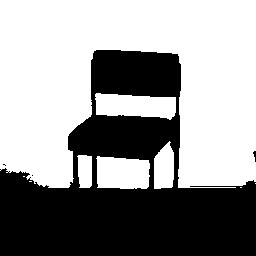
\includegraphics[width=0.15\textwidth]{img/res/e6/alg1agregadoowa1chair.jpg} &
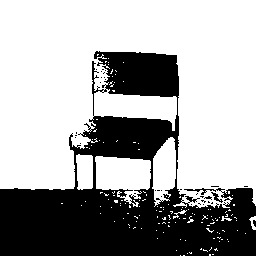
\includegraphics[width=0.15\textwidth]{img/res/e6/alg1agregadoowa2chair.jpg} &
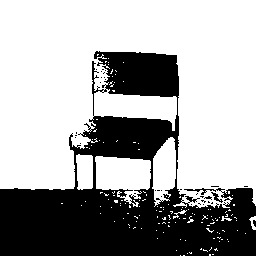
\includegraphics[width=0.15\textwidth]{img/res/e6/alg1agregadoowa3chair.jpg} \\\hline

\includegraphics[width=0.15\textwidth]{img/res/e6/alg1agregadoowa1block.jpg} &

\includegraphics[width=0.15\textwidth]{img/res/e6/alg1agregadoowa2block.jpg} &

\includegraphics[width=0.15\textwidth]{img/res/e6/alg1agregadoowa3block.jpg} \\\hline

\includegraphics[width=0.15\textwidth]{img/res/e6/alg1agregadoowa102.jpg} &

\includegraphics[width=0.15\textwidth]{img/res/e6/alg1agregadoowa202.jpg} &

\includegraphics[width=0.15\textwidth]{img/res/e6/alg1agregadoowa302.jpg} \\\hline
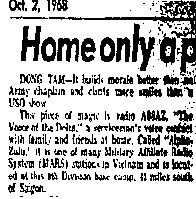
\includegraphics[width=0.15\textwidth]{img/res/e6/alg1agregadoowa109.jpg} &

\includegraphics[width=0.15\textwidth]{img/res/e6/alg1agregadoowa209.jpg} &

\includegraphics[width=0.15\textwidth]{img/res/e6/alg1agregadoowa309.jpg} \\\hline

\includegraphics[width=0.15\textwidth]{img/res/e6/alg1agregadoowa107.jpg} &

\includegraphics[width=0.15\textwidth]{img/res/e6/alg1agregadoowa207.jpg} &

\includegraphics[width=0.15\textwidth]{img/res/e6/alg1agregadoowa307.jpg} \\\hline
\end{tabular}
\caption{Resultados gráficos para la versión agregada del algoritmo 1 con la aplicación de OWA. \label{tab:resultexp6imagenes}}
\end{table}


Se presentan, también, los resultados de aplicar sobre imágenes con ruido. Se ve que, claramente, existe una tendencia de que la segunda forma de crear el OWA haga que el umbral se dispare hacia un extremo. Aun así, y de nuevo se puede apreciar claramente con la imagen segmentada de la tabla \ref{tab:resultexp6imagenesruido}, que la segmentación es bastante peor, sin contar el tiempo de computación extra que es necesario.

\begin{table}
\centering
\begin{tabular}{c||c|c|c} 
                         &\bb Media&\bb OWA (1)&\bb OWA (2)\\\hline\hline
\bb R. gausiano         &   131 &   56  &   0   \\\hline
\bb R. impulsivo 0,05   &   127 &   50  &   50  \\\hline
\bb R. impulsivo 0,2    &   136 &   50  &   50  \\\hline
\end{tabular}
\caption{Resultados gráficos para la versión agregada del algoritmo 1 con la aplicación de OWA.\label{tab:resultexp6ruido}}
\end{table}

\begin{table}
\centering
%\resizebox*{3\textwidth}{!}{
\begin{tabular}{c|c|c} 
\multicolumn{4}{c}{}\\
\bb Media&\bb OWA (1)&\bb OWA (2)\\\hline\hline
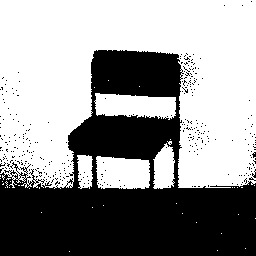
\includegraphics[width=0.15\textwidth]{img/res/e6/alg1agregadoowa1chairga.jpg} &
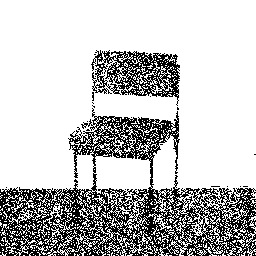
\includegraphics[width=0.15\textwidth]{img/res/e6/alg1agregadoowa2chairga.jpg} &

\includegraphics[width=0.15\textwidth]{img/res/e6/alg1agregadoowa3chairga.jpg} \\\hline
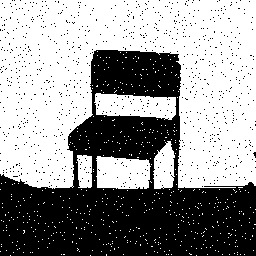
\includegraphics[width=0.15\textwidth]{img/res/e6/alg1agregadoowa1chairsp005.jpg} &
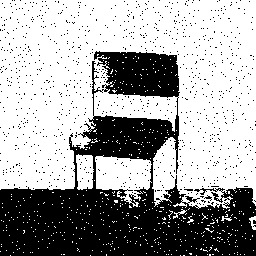
\includegraphics[width=0.15\textwidth]{img/res/e6/alg1agregadoowa2chairsp005.jpg} &
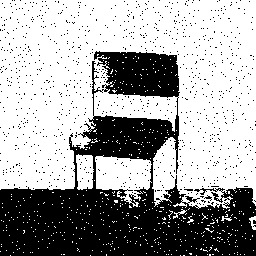
\includegraphics[width=0.15\textwidth]{img/res/e6/alg1agregadoowa3chairsp005.jpg} \\\hline
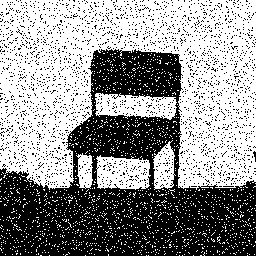
\includegraphics[width=0.15\textwidth]{img/res/e6/alg1agregadoowa1chairsp020.jpg} &
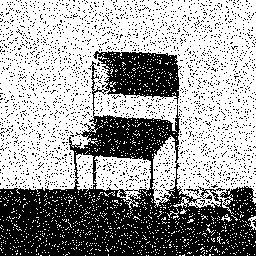
\includegraphics[width=0.15\textwidth]{img/res/e6/alg1agregadoowa2chairsp020.jpg} &
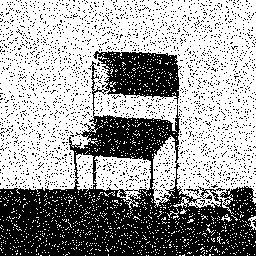
\includegraphics[width=0.15\textwidth]{img/res/e6/alg1agregadoowa3chairsp020.jpg} \\\hline
\end{tabular}
\caption{Resultados gráficos para la versión agregada del algoritmo 1 con la aplicación de OWA en imágenes con ruido.\label{tab:resultexp6imagenesruido}}
\end{table}


% EXPERIMENTO 7
\subsection{Experimento 7: sustitución de la media aritmética por funciones OWA en la construcción de los conjutos difusos para el algoritmo del umbral óptimo por similitud}
\subsubsection{Explicación del experimento}
En este caso, se cambiará la media aritmética que se encuentra en la creación del conjunto $H$ que se utiliza para conocer la similitud de las imágenes. Se mantendrá de esta forma durante todo el experimento. Únicamente cambiará la media que se encuentra en la creación de los conjuntos difusos que se comparan contra $H$.

Se distinguirán dos casos, por medio de las dos funciones OWA que se han explicado. Aquel que acoge a la OWA (1) es el Alg. 3 (a) y el que multiplica por el histograma será el Alg. 3 (b).

\subsubsection{Resultados}
De nuevo se vuelve a observar que no se dan buenos resultados para aquellas opciones que siguen que siguen teniendo la construcción del conjunto $Q_t$ por medio de OWA. En cambio, se observa un cambio muy interesante, ya que parece que la versión que se utiliza con la media aritmética pero con OWA para crear el conjunto H obtiene grandes resultados, para el caso en el cual no se multiplica por el histograma (Alg 3 (a)). Tampoco se desdiñen los resultados obtenidos con e OWA (2), la versión (b), aunque no son tan buenos.
%\REV{errores}
\begin{table}
\centering
\begin{tabular}{c||c|c|c}
Silla                                &\bb Media&\bb OWA (1)&\bb OWA (2)\\\hline\hline
\bb Alg. 3 (a)  &   119 &   50  &   50  \\\hline
                            
\bb Alg. 3 (b)  &   103 &   114 &   172 \\\hline
\multicolumn{4}{c}{}\\
Bloques                              &\bb Media&\bb OWA (1)&\bb OWA (2)\\\hline\hline
\bb Alg. 3 (a)     &   47  &   13  &   4   \\\hline
                            
\bb Alg. 3 (b)     &   30  &   11  &   65  \\\hline
\multicolumn{4}{c}{}\\
Engranaje                            &\bb Media&\bb OWA (1)&\bb OWA (2)\\\hline\hline
\bb Alg. 3 (a)  &   84  &   4   &   1   \\\hline
                            
\bb Alg. 3 (b)  &   147 &   89  &   193 \\\hline
\multicolumn{4}{c}{}\\
Letras                               &\bb Media&\bb OWA (1)&\bb OWA (2)\\\hline\hline
\bb Alg. 3 (a)  &   200 &   255 &   236 \\\hline
                            
\bb Alg. 3 (b)  &   178 &   171 &   168 \\\hline
\multicolumn{4}{c}{}\\
Sombra                               &\bb Media&\bb OWA (1)&\bb OWA (2)\\\hline\hline
\bb Alg. 3 (a)  &   121 &   255 &   85  \\\hline
                            
\bb Alg. 3 (b)  &   101 &   136 &   136 \\\hline
\end{tabular}
\caption{Umbrales para cada imagen con el algoritmo 3 a través la aplicación de OWA.\label{tab:resultexp7}}
\end{table}

\begin{table}
\centering
%\resizebox*{3\textwidth}{!}{
\begin{tabular}{c||c|c|c} 
\multicolumn{4}{c}{}\\
Silla                                &\bb Media&\bb OWA (1)&\bb OWA (2)\\\hline\hline
\bb Alg. 3 (a)  &  
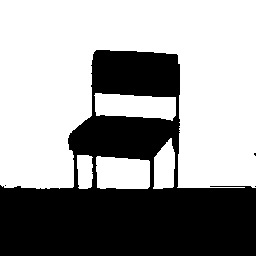
\includegraphics[width=0.12\textwidth]{img/res/e7/alg3aowa1chair.jpg} &
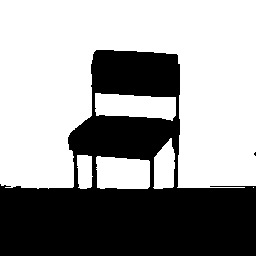
\includegraphics[width=0.12\textwidth]{img/res/e7/alg3aowa2chair.jpg} &
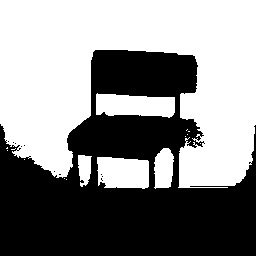
\includegraphics[width=0.12\textwidth]{img/res/e7/alg3aowa3chair.jpg} \\
\bb Alg. 3 (b)  &   
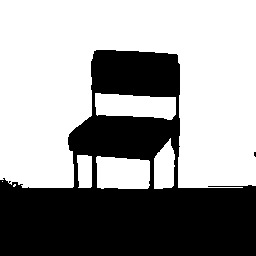
\includegraphics[width=0.12\textwidth]{img/res/e7/alg3bowa1chair.jpg} &
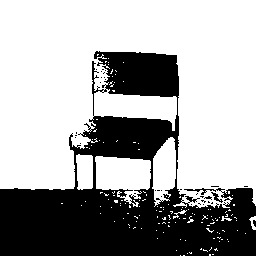
\includegraphics[width=0.12\textwidth]{img/res/e7/alg3bowa2chair.jpg} &
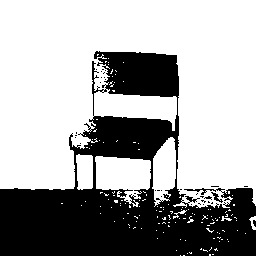
\includegraphics[width=0.12\textwidth]{img/res/e7/alg3bowa3chair.jpg} \\\hline
\multicolumn{4}{c}{}\\
Bloques                              &\bb Media&\bb OWA (1)&\bb OWA (2)\\\hline\hline
\bb Alg. 3 (a)  &  

\includegraphics[width=0.12\textwidth]{img/res/e7/alg3aowa1block.jpg} &

\includegraphics[width=0.12\textwidth]{img/res/e7/alg3aowa2block.jpg} &

\includegraphics[width=0.12\textwidth]{img/res/e7/alg3aowa3block.jpg} \\
\bb Alg. 3 (b)  &   

\includegraphics[width=0.12\textwidth]{img/res/e7/alg3bowa1block.jpg} &

\includegraphics[width=0.12\textwidth]{img/res/e7/alg3bowa2block.jpg} &

\includegraphics[width=0.12\textwidth]{img/res/e7/alg3bowa3block.jpg} \\\hline
\multicolumn{4}{c}{}\\
Engranaje                            &\bb Media&\bb OWA (1)&\bb OWA (2)\\\hline\hline
\bb Alg. 3 (a)  &  
\includegraphics[width=0.12\textwidth]{img/res/e7/alg3aowa102.jpg} &
\includegraphics[width=0.12\textwidth]{img/res/e7/alg3aowa202.jpg} &
\includegraphics[width=0.12\textwidth]{img/res/e7/alg3aowa302.jpg} \\
\bb Alg. 3 (b)  &   
\includegraphics[width=0.12\textwidth]{img/res/e7/alg3bowa102.jpg} &
\includegraphics[width=0.12\textwidth]{img/res/e7/alg3bowa202.jpg} &
\includegraphics[width=0.12\textwidth]{img/res/e7/alg3bowa302.jpg} \\\hline
\multicolumn{4}{c}{}\\
Letras                               &\bb Media&\bb OWA (1)&\bb OWA (2)\\\hline\hline
\bb Alg. 3 (a)  &  
\includegraphics[width=0.12\textwidth]{img/res/e7/alg3aowa109.jpg} &
\includegraphics[width=0.12\textwidth]{img/res/e7/alg3aowa209.jpg} &
\includegraphics[width=0.12\textwidth]{img/res/e7/alg3aowa309.jpg} \\
\bb Alg. 3 (b)  &   
\includegraphics[width=0.12\textwidth]{img/res/e7/alg3bowa109.jpg} &
\includegraphics[width=0.12\textwidth]{img/res/e7/alg3bowa209.jpg} &
\includegraphics[width=0.12\textwidth]{img/res/e7/alg3bowa309.jpg} \\\hline
\multicolumn{4}{c}{}\\
Sombra                               &\bb Media&\bb OWA (1)&\bb OWA (2)\\\hline\hline
\bb Alg. 3 (a)  &  
\includegraphics[width=0.12\textwidth]{img/res/e7/alg3aowa107.jpg} &
\includegraphics[width=0.12\textwidth]{img/res/e7/alg3aowa207.jpg} &
\includegraphics[width=0.12\textwidth]{img/res/e7/alg3aowa307.jpg} \\
\bb Alg. 3 (b)  &   
\includegraphics[width=0.12\textwidth]{img/res/e7/alg3bowa107.jpg} &
\includegraphics[width=0.12\textwidth]{img/res/e7/alg3bowa207.jpg} &
\includegraphics[width=0.12\textwidth]{img/res/e7/alg3bowa307.jpg} \\\hline
\end{tabular}
\caption{Resultados gráficos para el algoritmo 3 con la aplicación de OWA.\label{tab:resultexp7imagenes}}
\end{table}

En el caso de las imágenes con ruido, la tendencia es exactamente la misma. Como ha ocurrido en todos los experimentos, no se diluye el ruido ya que con un umbral este no puede desaparecer. Esto se se muy claro en el ruido impulsivo. Se solucionaría con un filtro.

\begin{table}
\centering
\begin{tabular}{c||c|c|c}
R. gausiano                         &\bb Media&\bb OWA (1)&\bb OWA (2)\\\hline\hline
\bb Alg. 3 (a)  &   132 &   56  &   0   \\\hline
                            
\bb Alg. 3 (b)  &   99  &   154 &   159 \\\hline
\multicolumn{4}{c}{}\\
R. impulsivo 0,05                    &\bb Media&\bb OWA (1)&\bb OWA (2)\\\hline\hline
\bb Alg. 3 (a)  &   144 &   50  &   50  \\\hline
                            
\bb Alg. 3 (b)  &   111 &   122 &   172 \\\hline
\multicolumn{4}{c}{}\\
R. impulsivo 0,2                     &\bb Media&\bb OWA (1)&\bb OWA (2)\\\hline\hline
\bb Alg. 3 (a)     &   152 &   50  &   0   \\\hline
                            
\bb Alg. 3 (b)     &   127 &   131 &   172 \\\hline
\end{tabular}
\caption{Umbrales para cada imagen con el algoritmo 3 a través la aplicación de OWA en imágenes con ruido.\label{tab:resultexp7ruido}}
\end{table}

\begin{table}
\centering
\begin{tabular}{c||c|c|c} 
\multicolumn{4}{c}{}\\
R. gausiano                                 &\bb Media&\bb OWA (1)&\bb OWA (2)\\\hline\hline
\bb Alg. 3 (a)  &  
\includegraphics[width=0.12\textwidth]{img/res/e7/alg3aowa1chairga.jpg} &
\includegraphics[width=0.12\textwidth]{img/res/e7/alg3aowa2chairga.jpg} &
\includegraphics[width=0.12\textwidth]{img/res/e7/alg3aowa3chairga.jpg} \\
\bb Alg. 3 (b)  &   
\includegraphics[width=0.12\textwidth]{img/res/e7/alg3bowa1chairga.jpg} &
\includegraphics[width=0.12\textwidth]{img/res/e7/alg3bowa2chairga.jpg} &
\includegraphics[width=0.12\textwidth]{img/res/e7/alg3bowa3chairga.jpg} \\\hline
\multicolumn{4}{c}{}\\
R. impulsivo 0,05                             &\bb Media&\bb OWA (1)&\bb OWA (2)\\\hline\hline 
\bb Alg. 3 (a)  &  
\includegraphics[width=0.12\textwidth]{img/res/e7/alg3aowa1chairsp005.jpg} &
\includegraphics[width=0.12\textwidth]{img/res/e7/alg3aowa2chairsp005.jpg} &
\includegraphics[width=0.12\textwidth]{img/res/e7/alg3aowa3chairsp005.jpg} \\
\bb Alg. 3 (b)  &   
\includegraphics[width=0.12\textwidth]{img/res/e7/alg3bowa1chairsp005.jpg} &
\includegraphics[width=0.12\textwidth]{img/res/e7/alg3bowa2chairsp005.jpg} &
\includegraphics[width=0.12\textwidth]{img/res/e7/alg3bowa3chairsp005.jpg} \\\hline
\multicolumn{4}{c}{}\\
R. impulsivo 0,2                        &\bb Media&\bb OWA (1)&\bb OWA (2)\\\hline\hline
\bb Alg. 3 (a)  &  
\includegraphics[width=0.12\textwidth]{img/res/e7/alg3aowa1chairsp020.jpg} &
\includegraphics[width=0.12\textwidth]{img/res/e7/alg3aowa2chairsp020.jpg} &
\includegraphics[width=0.12\textwidth]{img/res/e7/alg3aowa3chairsp020.jpg} \\
\bb Alg. 3 (b)  &   
\includegraphics[width=0.12\textwidth]{img/res/e7/alg3bowa1chairsp020.jpg} &
\includegraphics[width=0.12\textwidth]{img/res/e7/alg3bowa2chairsp020.jpg} &
\includegraphics[width=0.12\textwidth]{img/res/e7/alg3bowa3chairsp020.jpg} \\\hline
\end{tabular}
\caption{Resultados gráficos para el algoritmo 3 con la aplicación de OWA en imágenes con ruido.\label{tab:resultexp7imagenesruido}}
\end{table}


\chapter{Conclusiones y líneas de futuro}\label{cap:conclusiones}
\section{Conclusiones}
\section{Líneas de futuro}

%\noappendicestocpagenum
%\appendixpage
%\addappheadtotoc
%\appendix
% Adjustments headers
%\pagestyle{fancy}
%\fancyhead[LO]{\leftmark}
%\ifdefined\euskaraz
%	\fancyhead[RE]{\emph{\thechapter eranskina}}
%\else
%	\fancyhead[RE]{\emph{Anexo \thechapter}}
%\fi
%\renewcommand{\headrulewidth}{0.5pt}

% \chapter{Implementaciones de los algoritmos}

\section{Algoritmo general maximizando la similitud}

%\noident
\begin{listing}\label{cod:alg1}
\matlabfile{codigo/alg1.m}

    \caption{Esto es una prueba}
\end{listing}

\section{Algoritmo del área}
\section{Algoritmo de selección del umbral óptimo}
\section{Algoritmo de umbralización global}
\section{Algoritmo de Otsu}
\section{Algoritmo de maximización de la entropía de Renyi}
\section{Algoritmo {\em k-means}}

%\backmatter

%\bibliographystyle{ieeetr} % Use the "unsrtnat" BibTeX style for formatting the Bibliography
%\bibliographystyle{babamspl}
%\bibliography{bibliografia}
\nocite{*}
\printbibliography[heading=bibintoc]
%\bibliography{bibliografia}{} % The references (bibliography) information are stored in the file named "Bibliography.bib"

% In case we are using a glossary
% \glstoctrue
% \glsaddall
% \printglossaries

\end{document}